\documentclass[10pt, a4paper]{article}
\usepackage[ngerman]{babel}
\usepackage[utf8]{inputenc}
\usepackage[T1]{fontenc}
\usepackage{xcolor}
\usepackage{hyperref}
\usepackage{comment}
\usepackage{enumitem}
\usepackage[backend=biber,style=alphabetic,]{biblatex}
\usepackage{csquotes}
\usepackage{graphicx}
\usepackage{wrapfig}
\usepackage{listings}
\usepackage[onehalfspacing]{setspace}

\definecolor{lightgray}{rgb}{.9,.9,.9}
\definecolor{darkgray}{rgb}{.4,.4,.4}
\definecolor{purple}{rgb}{0.65, 0.12, 0.82}
\lstdefinelanguage{TypeScript}{
  keywords={typeof, new, true, false, catch, function, return, null, catch, switch, var, if, in, while, do, else, case, break, string, number, boolean},
  keywordstyle=\color{blue}\bfseries,
  ndkeywords={class, export, boolean, throw, implements, import, this},
  ndkeywordstyle=\color{purple}\bfseries,
  identifierstyle=\color{black},
  sensitive=false,
  comment=[l]{//},
  morecomment=[s]{/*}{*/},
  commentstyle=\color{green}\ttfamily,
  stringstyle=\color{red}\ttfamily,
  morestring=[b]',
  morestring=[b]"
}

\lstset{
  frame=single,
  language=TypeScript,
  keywordstyle=\color{blue},
  commentstyle=\color{green},
  numbers=left,
  numberstyle=\tiny,
  basicstyle=\footnotesize\ttfamily,
  showstringspaces=false,
  breaklines=true,
  xleftmargin=.04\textwidth,
  commentstyle=\color{blue},
}

\lstset{literate=
    {á}{{\'a}}1 {é}{{\'e}}1 {í}{{\'i}}1 {ó}{{\'o}}1 {ú}{{\'u}}1
    {Á}{{\'A}}1 {É}{{\'E}}1 {Í}{{\'I}}1 {Ó}{{\'O}}1 {Ú}{{\'U}}1
    {à}{{\`a}}1 {è}{{\`e}}1 {ì}{{\`i}}1 {ò}{{\`o}}1 {ù}{{\`u}}1
    {À}{{\`A}}1 {È}{{\'E}}1 {Ì}{{\`I}}1 {Ò}{{\`O}}1 {Ù}{{\`U}}1
    {ä}{{\"a}}1 {ë}{{\"e}}1 {ï}{{\"i}}1 {ö}{{\"o}}1 {ü}{{\"u}}1
    {Ä}{{\"A}}1 {Ë}{{\"E}}1 {Ï}{{\"I}}1 {Ö}{{\"O}}1 {Ü}{{\"U}}1
    {â}{{\^a}}1 {ê}{{\^e}}1 {î}{{\^i}}1 {ô}{{\^o}}1 {û}{{\^u}}1
    {Â}{{\^A}}1 {Ê}{{\^E}}1 {Î}{{\^I}}1 {Ô}{{\^O}}1 {Û}{{\^U}}1
    {Ã}{{\~A}}1 {ã}{{\~a}}1 {Õ}{{\~O}}1 {õ}{{\~o}}1
    {œ}{{\oe}}1 {Œ}{{\OE}}1 {æ}{{\ae}}1 {Æ}{{\AE}}1 {ß}{{\ss}}1
    {ű}{{\H{u}}}1 {Ű}{{\H{U}}}1 {ő}{{\H{o}}}1 {Ő}{{\H{O}}}1
    {ç}{{\c c}}1 {Ç}{{\c C}}1 {ø}{{\o}}1 {å}{{\r a}}1 {Å}{{\r A}}1
    {€}{{\euro}}1 {£}{{\pounds}}1 {«}{{\guillemotleft}}1
    {»}{{\guillemotright}}1 {ñ}{{\~n}}1 {Ñ}{{\~N}}1 {¿}{{?`}}1
}%\'

\usepackage{caption}
\DeclareCaptionFormat{citation}{%
   \ifx\captioncitation\relax\relax\else
     \captioncitation\par
   \fi
   #1#2#3\par}
\newcommand*\setcaptioncitation[1]{\def\captioncitation{\textit{Source:}~#1}}
\let\captioncitation\relax
\captionsetup{format=citation,justification=centering}
\graphicspath{ {./images/} }


\addbibresource{literature.bib}

\title{Projektbericht Smart Music Player}
\author{Anton Bracke\\Jan Eberlein\\Tom Calvin Haak\\Julian Hahn\\Nick Loewecke}

\newsavebox\curwrapfig
\makeatletter
\long\def\wrapfiguresafe#1#2#3#4{%
  \sbox\curwrapfig{#3}%
  \par\penalty-100%
  \begingroup % preserve \dimen@
    \dimen@\pagegoal \advance\dimen@-\pagetotal % space left
    \advance\dimen@-\baselineskip % allow an extra line
    \ifdim \ht\curwrapfig>\dimen@ % not enough space left
      \break%
    \fi%
  \endgroup%
  \begin{wrapfigure}{#1}{#2}%
    \usebox\curwrapfig%
    \caption{#4}
  \end{wrapfigure}%
}
\makeatother

\begin{document}
\begin{onehalfspace}
\maketitle
\newpage
\tableofcontents
\newpage

%\begin{lstlisting}[caption={CAPTION_GOES_HERE}, captionpos=b]
  %Code code code
%\end{lstlisting}

%\wrapfiguresafe{r}{0mm}{\includegraphics[width=4cm]{IMAGENAME.EXT}}{IMAGE_DESCRIPTION}


\section{Einleitung}
Ein zentraler Teil des Studiengangs \glqq Informationstechnologie\grqq{} ist es, Softwareentwicklung in Teams und Kommunikation mit Kund:innen zu erlernen. \cite{Qualifikationsziele_Informationstechnologie}
Dies passiert vor allem im Modul \glqq Projekt Informatik (PROI)\grqq{}.
In diesem arbeiten Studierende ein Semester lang in kleinen Gruppen an verschiedenen Projekten.
Diese bilden häufig reale Sachverhalte der Softwareentwicklung ab und werden meist von Firmenpartner:innen aus der Wirtschaft gestellt.
Die Teams wählen ein oder mehrere Projekte, die sie gerne bearbeiten würden, und stellen sich mit einer Kurzbewerbung bei den entsprechenden Firmen vor.
Welche Teams die jeweiligen Projekte bearbeiten, entscheiden die Firmen selbst.
\\
Dieser Bericht beschreibt das Projekt und dessen Verlauf, dass das Autoren-Team für die macio GmbH aus Kiel bearbeitete.

\subsection{Unternehmen}
Das Unternehmen macio stellte in ihrer Ausschreibung als einzige Firma die Anforderung, dass Projekt quelloffen (\textit{Open Source}) umzusetzen.
Das Team schätzte die Bereitschaft, die geleistete Arbeitszeit nicht für den Eigenbedarf zu nutzen, sondern einen Beitrag für die Open-Source-Community zu leisten.
Damit wurde die folgende Definition für Open-Source erfüllt:

\begin{quote}
  \textit{Ich denke, dass jede allgemein nützliche Information frei sein sollte.
  Mit 'frei' beziehe ich mich nicht auf den Preis, sondern auf die Freiheit, Informationen zu kopieren und für die eigenen Zwecke anpassen zu können.
  Wenn Informationen allgemein nützlich sind, wird die Menschheit durch ihre Verbreitung reicher, ganz egal, wer sie weiter gibt und wer sie erhält.}
  \cite{openSource}
\end{quote}

Das Hauptgeschäft von macio ist das Design und Entwickeln von Mensch-Maschine-Interfaces.
Als etabliertes Unternehmen konnten Sie neben der Rolle des Kunden auch ihre jahrelange Erfahrung bei Bedarf einbringen und Hilfestellung leisten.
So gab beispielsweise ein Designer des Unternehmens hilfreiches Feedback zum Entwurf der Benutzeroberfläche.
\subsection{Anforderungsanalyse}
Im Rahmen des Projekt Informatik möchte Macio ihr Portfolio im IoT-Bereich erweitern, sowie ihren Empfangsraum im Standort Kiel verschönern.
Hierfür soll eine smarte Spielzeug-Box gebaut werden.
Da die aktuell am Markt erhältlichen Konkurrenzprodukte wenig konfigurierbarkeit bieten, zum Beispiel kein anderer Lautsprecher ausgewählt werden kann, sollte hier eine Open-Source Alternative geschaffen werden, die dem Nutzer volle Freiheiten zur Anpassung bietet.
\subsubsection{Produktvision}
Mithilfe der von macio gestellten Projektskizze (siehe \ref{pdf:macioprojektskizze}) erstellte das Team die folgende Produktvision:
Angestrebt wurde die Konzeption und Entwicklung einer Musik-Box, die NFC Tags lesen kann und Schnittstellen zu Musik-Streaming-Anbietern (wie Spotify) besitzt.
Wird auf die Box beispielsweise ein Spielzeuge (z.B. in Form von kleinen Figuren) mit integrierten NFC-Chips gestellt, soll ein frei konfigurierbares Musikstück über eine bereits bestehende Musik-Anlage abgespielt abgespielt werden.
Falls es im Rahmen des Projektes möglich ist, sollen die Nutzer in der Lage sein, zwischen verschiedenen Musikanbietern zu wechseln.
NFC-Chips und die zugehörige Musik sollen über ein Web-basierte Benutzeroberfläche konfiguriert werden können.
Diese Benutzeroberfläche soll von der Box ausgeliefert und primär für Smartphone-Bedienung gestaltet werden.
Da es sich um ein Open Source Projekt mit entsprechender Lizenz handelt, muss auch eine aussagekräftige, öffentliche Dokumentation verfasst werden.
Macio stellte die benötigte Hardware zur Verfügung und unterstützte bei technischen Fragen.\\

\subsubsection{Anforderungen}
Aus der Projektskizze und der Produktvision wurden folgende konkrete Mindestanforderungen und entsprechende Klassifikationen an das Produkt abgeleitet:
\begin{center}
  \begin{table}[h!]
    \begin{tabular}{c|c}
      Anforderung & Klassifikation\\
      \hline
      NFC-Tags lesen, schreiben und entschlüsseln & funktional  \\
      Mit Spotify Connect verbinden und arbeiten & funktional \\
      Responsive UI konzeptionieren und umsetzen & funktional  \\
      Aussagekräftige Dokumentation mit Benutzerhandbuch & nicht funkt.  \\
    \end{tabular}
    \caption{\label{mind-anforderungen}Mindestanforderungen}
\end{table}
\end{center}

Um diese Anforderungen weiter zu definieren erstellte das Team User Stories,
durch die sichergestellt wurde, dass beide Parteien (der Kunde und die Entwickler) die Anforderungen  gleich interpretierten und verstanden.
Dabei entstand auch eine Priorisierung der Anforderungen, bemessen an dem \textit{Return of Investment} und dem Nutzen für den Endnutzer.
Im weiteren Gespräch mit den Kunden ergaben sich ergänzende Anforderungen an das Produkt:
\begin{center}
  \begin{table}[h!]
    \begin{tabular}{c|c}
    Anforderung & Klassifikation \\
    \hline
    Sound Wiedergabe auf der Box selbst & funktional  \\
    Unterstützung anderer Musikdienste & funktional \\
    3D-Modellierung und Print einer passenden Box & nicht funkt.  \\
    Maximaler Kostenpunkt von 30€ & nicht funkt.  \\
    Cloud-Anbindung der Box & funktional \\
    Auslieferung des UI aus der Cloud & funktional \\
    \end{tabular}
    \caption{\label{erg-anforderungen}ergänzende Anforderungen}
  \end{table}
\end{center}

Durch die agile Projektorganisation wuchsen diese Anforderungen iterativ von Sprint zu Sprint und neue implizite Anforderungen entstanden.
Um die Kosten von maximal 30€ zu realisieren, entstand die Idee zur Konzeption von zwei Versionen der \textit{Leek-Box}. Während die kostengünstige Variante nur die Grundfunktionen umsetzt, bietet die teurere einen größeren Funktionsumfang, wie das Abspielen der Musik über einen eigenen Lautsprecher.
Einige der Anforderungen haben sich während der Entwicklungsphase als widersprüchlich herausgestellt.
So wurde sich zum Beispiel gegen bezahlte Services entschieden. Dies schränkte die Usability ein, entsprach jedoch mehr dem Open-Source-Gedanken des Projekts.
Ob und wie diese Anforderungen umgesetzt werden können wird im späteren Abschnitt Machbarkeitsstudie (Abschnitt \ref{machbarkeitsstudie}) behandelt.

\section{Projektplanung}
  \subsection{Projekt Management}
  Am Anfang des Projekt entschied sich das Team in Abstimmung mit macio für eine agile Projektorganisation.
  Diese Richtung des Projektmanagements zeichnet sich vor allem durch fortlaufende Produktentwicklung, kontinuierliches Feedback, kooperatives Arbeiten und
  Reaktionsfähigkeit bei Anforderungsänderungen aus. Diese Entscheidung geschah aus mehreren Gründen.
  Zum einen haben agile Methoden kein festes Endprodukt als Ziel, wie es beispielsweise bei klassischer Softwareentwicklung
  (Wasserfallmodell, V-Model, etc) der Fall ist. Solch ein festes Ende würde der geforderten Veröffentlichung als Open-Source-Projekt nicht gerecht werden,
  da solche per Definition erweiterbar sind. Des Weiteren haben agile Entwicklungsprozesse vergleichsweise kürzere Veröffentlichungszyklen,
  was dem Team ermöglichte, ein funktionierendes Produkt innerhalb des recht knappen Zeitrahmens eines
  Semesters\footnote{Dieses Semester war aufgrund besonderer CoViD19-bedingten Auflagen einige Wochen kürzer als ein typisches.} zu erstellen.
  \\
  Entsprechend der Entscheidung zu agiler Entwicklung wurde zu Beginn des Projekt keine feste Planung des Projektverlaufs aufgestellt.
  Stattdessen entwickelte das Team eine Methodik um iterativ am Projekt zu arbeiten, wobei sich an der Methode Scrum orientiert wurde.
  Aus dieser wurden vor allem die Einteilung in Projektiterationen fester Länge (Sprints) und die zugehörigen wiederkehrenden Meetings übernommen.
  Diese Sprintlänge betrug im allgemeinen zwei Wochen\footnote{Abgewichen wurde von dieser Länge nur zum Jahresende, um die Feiertage unterzubringen.}.
  Die Rollen der Teammitglieder in Scrum wurde nicht adaptiert, da sich im Team für eine Gleichverteilung der Aufgaben entschieden wurde.

  \subsection{Vor den Sprints}
  Den Anfang eines jeden Sprints stellte das Sprint-Planing dar.
  Im diesem stellte das Team eine Vision für die Sprintiteration auf.
  Diese wurde gemeinsam mit dem Kunden abgesprochen und gegebenenfalls abgeändert.
  Im Anschluss wurde die Produktvision vom Team in technisch orientierte Arbeitspakete aufgeteilt.
  Dies geschah anhand des geschätzten zeitlichen Arbeitsaufwands der einzelnen Änderungen.
  Falls sich hierbei gegebenenfalls herausstellte, dass einzelne Arbeitspakete nicht umsetzbar oder zu aufwändig waren, wurde die Produktvision entsprechend angepasst.


  \subsection{Arbeit in den Sprints}
  Während der Sprints wurde die Produktvision aus den Sprint-Planings implementiert.
  Alle Mitglieder des Team waren an dieser Arbeit beteiligt.
  Die einzelnen Arbeitspakete wurden entweder alleine, in Paaren oder selten auch in Gruppen bearbeitet.
  Dies wurde anhand der Anforderung und des Aufwands der jeweiligen Arbeitspakete entschieden.
  Auch das spezifische Fachwissen der beteiligten Personen hatte einen Einfluss auf die Aufteilung.
  In jedem Fall wurden die Pakete erst bei Arbeitsbeginn und nur von den bearbeitenden Mitgliedern selbst zugewiesen.
  \\
  Nach Bearbeitung eines Paketes wurden die vollzogenen Änderungen durch Code Reviews von mindestens zwei anderen Entwicklern geprüft.
  Nur wenn diese erfolgreich waren, wurde der entsprechende Code ins Produktinkrement übernommen.
  Dieses Verfahren wurde angesetzt, um sowohl Flexibilität von Arbeitszeiten zu ermöglichen, als auch um die gewünschte Produktqualität sichherzustellen.
  Verschiedene Arbeitszeiten waren notwendig, da alle Teammitglieder verschiedene parallele Veranstaltungen besuchten und anderen beruflichen Tätigkeiten nachgingen.
  So waren keine langfristigen synchronen Arbeitszeiten aller Mitglieder möglich.
  Die freie Verteilung von Paketen ermöglichte auch, dass Mitglieder in persönlich bevorzugten Themengebieten arbeiten konnten.
  Dies half die Motivation des Teams am Projekt hochzuhalten.
  \\
  Um sich während der Sprints abzustimmen und um Arbeitsfortschritte abzugleichen, trafen sich die Teammitglieder drei Mal pro Woche.
  Dies geschah immer montags, mittwochs und freitags.
  Bei Bedarf wurde auch von dieser Taktung abgewichen.
  In Aufbau und Zweck orientierten sich diese regelmäßigen Meetings an den \glqq Daily Standups\grqq{} der Scrum-Methode.
  Während den Meetings stellte jedes Teammitglied kurz vor was es seit dem letzten Standup am Projekt bearbeitet hatte, welche Probleme dabei aufgetreten waren und was bei der Arbeit gelernt wurde.
  Auch welche Themen jedes Mitglied bis zum nächsten Standup bearbeiten wollte, wurde besprochen.
  Nach diesen Kurzvorstellungen wurden einzelne besonders interessante und wichtige Punkte der Arbeit oder gelöste Probleme im Detail besprochen.
  So konnte das Team auf den gleichen Wissensstand kommen und gemeinsam Entscheidungen treffen.

  \subsection{Am Ende der Sprints}
  Nach jedem Sprint wurde das Ergebnis bzw. das Produktinkrement dem Kunden und der Projektbetreuung vorgestellt.
  Hier wurde meist auch zusammen mit macio das Ausmaß des nächsten Produktinkrements besprochen.
  Die resultierenden Wünsche und Rückmeldungen wurden mit ins Backlog und die folgenden Besprechungen mitgenommen.
  Im Anschluss fand immer eine Retrospektive statt.
  In dieser besprach das Team die eigene Zusammenarbeit und den gemeinsamen Umgang.
  Hierfür stellten sich alle Teammitglieder für sich folgende Fragen für die Arbeit am entsprechenden Sprint:
  \begin{itemize}[noitemsep,topsep=0pt,parsep=0pt,partopsep=0pt]
    \item Was lief gut?
    \item Was lief schlecht?
    \item Was habe ich neu gelernt?
    \item Was können wir in Zukunft besser machen?
  \end{itemize}
  Die jeweiligen Antworten wurden zusammengetragen und im Team gemeinsam reflektiert.
  Das Feedback in diesem Kontext war konstruktiv und fair aber auch ehrlich.
  Die daraus entstandenen Erkenntnisse und Verbesserungsvorschläge wurden genutzt um das Teamwork und die Arbeit im folgenden Sprint weiter zu optimieren.
  Direkt nach jeder Retrospektive startete der nächste Sprint beginnend mit dem entsprechenden Sprint-Planing.

  \subsection{Quelloffenes Arbeiten}
  Teil der Anforderung war, dass die Software als Open-Source-Projekt der Öffentlichkeit zur Verfügung stehen soll.
  Dementsprechend entwickelte das Team den Anspruch, das dieses Projekt nicht nur Open-Source sondern auch erweiterbar und verständlich sein soll.
  Aufgrunddessen wurde die Entscheidung getroffen, das Projekt von Entwicklungsbeginn öffentlich auf GitHub aufzusetzten.
  Diese Platform bot sich an, da sie für den Umfang des Projekts viele hilfreiche Funktionalitäten in den Bereichen Automatisierung und Kollaboration bietet, allerdings trotzdem kostenlos ist
  Diese Werkzeuge halfen dabei den Entwicklungsprozess sehr intuitiv und zentral zu gestalten.
  So wurden zum Beispiel die meisten Diskussionen zu fachlichen Themen direkt in den Arbeitspaketen.
  Auch im Nachhinein können dann Entscheidungen und Denkprozesse von anderen Kollaborierenden nachvollzogen werden.
  Dies hilft zusätzlich bei der zukünftigen Instandhaltung und Weiterentwicklung des Projekts.
  \\
  Das Produkt-Backlog wurde auch in dieses GitHub Repository eingepflegt.
  Dies erhöhte einerseits die Übersichtlichkeit über den Stand des Projekts innerhalb, da Arbeitspakete und zugehöriger Code sehr einfach verknüpft werden konnten.
  Andererseits ermöglicht diese Zusammenlegung auch, dass andere Entwickler:innen einfach ins Projekt einsteigen und ihre Arbeit dokumentieren können, ohne andere Plattformen aufsuchen zu müssen.
  Die Möglichkeiten der Automatisierung wurden genutzt, um den Workflow zu vereinfachen und um die Code-Qualität sicherzustellen.
  Dies geschah zum Beispiel die durch die automatische Erstellung von Branches für einzelne Arbeitspakete bei Beginn der Bearbeitung und automatische statische und dynamische Tests des Codes.
  \\
  Darüber hinaus war die Open-Source Anforderung auch hilfreich bei der Produktentwicklung.
  So konnte die Zielgruppe für dieses Projekt auf Menschen mit fortgeschrittenen Technikkenntnissen und Interesse an Bastelprojekten eingeschränkt werden.
  Dies war vor allem für das erstmalige Einrichten und die zugehörige Dokumentation maßgebend.
  Entsprechend konnte sich hier eher technischer Sprache bedient werden.
  Allerdings galt diese Einschränkung der Zielgruppe auch nicht für alle Breiche des Projekts.
  Die Benutzbarkeit der Nutzeroberfläche sollte einfach und ohne Vorkenntnisse möglich sein, da die Musikbox z. B. verschenkt oder in Familien genutzt werden könnte.
  Dieser Anwendungsfall schließt andere Nutzende ein, als bei der Einrichtung.


\section{Machbarkeitsstudie}
\label{machbarkeitsstudie}

\subsection{NFC Tag}
\colorbox{orange}{lesen und schreiben vlt als ein gemeinsamer Abschnitt}
\colorbox{orange}{kurzer text der zu NFC-Tags allgemein schreibt}
\subsubsection*{lesen}
Um mit NFC Tags arbeiten zu können, müssen diese auch entschlüsselt bzw. gelesen werden können.
Hierfür ist ein Hardware NFC-Reader notwendig, der die Daten ausliest und an die Box kommuniziert.
Dieser emuliert dafür Keyboard Eingaben, die die Tag-IDs darstellen.
\textit{Evdev}, ein Kernel Modul von Linux, könnte dann zum Abgreifen dieser Keyboard-Eingaben genutzt werden. Mit \textit{node-evdev}\footnote{https://github.com/sdumetz/node-evdev} kann \textit{evdev} auch mit Node genutzt werden. Mit dem Fork\footnote{https://github.com/anbraten/node-evdev} von Anbraten wird zusätzlich der Raspberry Pi und die Typescript Unterstützung zur Verfügung gestellt.

\subsubsection*{schreiben}
Ein NFC-Tag hat generell eine feste ID.
Um weitere Daten auf einen NFC-Tag schreiben zu können, benötigt der NFC-Tag also einen eigenen Speicher.
Ist dieser vorhanden, können dort z.b. Kontaktdaten hinterlegt werden. Werden diese dann von einem Smartphone gelesen, öffnet sich die Kontakte-App und der auf dem NFC-Tag gespeicherte Kontakt kann abgespeichert werden.
Dafür wäre einerseits ein spezieller NFC-Reader, der auch schreiben kann, sowie eine spezielle Library notwendig.

\subsection{Raspberry Pi}
\subsubsection{Docker Integration}
\colorbox{orange}{warum Docker? warum virtualisierung?}
Auf einem Raspberri Pi Docker zu installieren und zum Laufen zu bringen wird in vielen Anleitungen online beschrieben\footnote{https://phoenixnap.com/kb/docker-on-raspberry-pi}.

\subsubsection{Öffentlich zugängliches Web Interface}
Auf einem Raspberry Pi könnte eine Web Anwendung gehosted werden, welche die allgemeine Web Anwendung für alle Boxen darstellen soll.
Um diese Web Anwendung von außerhalb des eigenen Netzwerkes erreichen zu können, muss innerhalb des Routers ein Port ge-forwarded werden.
Dann kann der Pi und dessen Webinterface unter der öffentlichen IP xxx.xxx.xxx.xxx des Routers erreicht werden.
Da sich die öffentliche IP-Adresse eines privaten Internet-Anschlusses in der Regel täglich ändert, wird zum einfachen finden der IP ein DynDns Service benötig, welcher eine feste Domain in die wechselnde IP Adresse des Routers übersetzt.
Alternativ ginge es auch ohne Port-Forwarding mit nginx und ngrok \footnote{https://vatsalyagoel.com/setting-up-a-public-web-server-using-a-raspberry-pi-3/}.
\colorbox{orange}{warum die? wofür sind die?}
Für Unerfahrene wären diese notwendingen Schritte zu Beginn etwas komplexere Thematiken. Der effektive Arbeitsaufwand hängt daher auch sehr stark von der Erfahrung der einzelnen Teammitglieder ab.

\subsubsection{URL für UI festlegen}
\colorbox{orange}{warum ist das interassant?}
Über ein mDNS Service, der auf dem Raspberri Pi läuft, wäre es möglich für die statische Public-IP eine eigene URL anzulegen.
Dafür sind verschiedene mDNS Services möglich, potentiell ist auch eine Domain notwendig.

\subsection{User Interface}
\subsubsection{Zugriff auf NFC Reader von Cloud Anwendung}
Um von der App auf die Daten vom NFC-Reader der verschiedenen Boxen zuzugreifen, wäre ein zentrales Backend mit einer API sinnvoll.
Der Computer der Box könnte beim Lesen eines NFC-Tag Daten über einen API Call an die Cloud Anwendung schicken, sodass die zusätzlich zu dem Backend verbundene App das gewünschte Event triggern kann.

\subsubsection{Login via Spotify, Youtube, etc.}
\colorbox{orange}{warum so? was ist die Alternative?}
Es gibt ein Feathers Plugin, welches die Möglichkeit bietet OAuth Provider zu nutzen, um sich über andere Services wie Spotify anzumelden.

\subsubsection{Nutzer verschiedener Streaminganbieter wiedererkennen}
Um gleiche Nutzer zu erkennen, müssten Merkmale angelegt werden, über die diese Nutzer wiedererkennbar wären.
Die E-Mail wäre hierbei ein geeignetes Merkmal, da dies einzigartig ist. Über gesetzte Scopes in der OAuth Anfrage kann diese vom jeweiligen Provider mitgeliefert werden.
Um die E-Mail als Wiedererkennungsmerkmal zu verwenden, muss vorausgesetzt sein, dass Nutzer immer die gleiche E-Mail bei den unterschiedlichen Providern nutzen. Dies ist aber nicht immer der Fall.
Daher könnte dem (bereits eingeloggten) Nutzer die Möglichkeit gegeben werden, weitere Accounts zu dem bestehenden hinzuzufügen und entsprechend in der Datenbank zu hinterlegen.

\subsubsection{Musik Artwork laden}
\colorbox{orange}{weniger umgangssprachlich und mehr}
Sollte bei der Verwendung von Spotify kein Problem sein, da zu jeder Anfrage von Titeln oder Liedern auch eine Liste von Bildern enthalten ist.\footnote{https://stackoverflow.com/questions/10123804/retrieve-cover-artwork-using-spotify-api}

\subsubsection{Eigene Bilder hochladen}
Eigene Bilder hochzuladen sollte möglich sein. In unserem Kontext mit Vue.js und Node.js würde das Plugin \textit{vue-picture-input} helfen.
Mit einem Axios Post könnte das Bild an das Backend gesendet werden. \footnote{https://www.digitalocean.com/community/tutorials/vuejs-uploading-vue-picture-input}

\subsubsection{Spotify Connect Lautsprecher auswählen}
\colorbox{orange}{spotify als einen Abschnitt und zu den anderen Services}
Das Auswählen von einem spezifischen Spotify Connect Lautsprecher ist möglich.
Über einen API Call an die Spotify API mit dem Endpunkt \textit{/v1""/me""/player""/device} wird eine Liste von allen verbundenen Geräten geliefert. Über den Endpunkt kann ein entsprechendes Lied zum Abspielen über den jeweiligen \textit{Spotify Connected Speaker} übergeben werden.
Sollte nicht explizit ein Lautsprecher angegeben werden, so wird der zuletzt aktive genutzt. Dieser hat bei \textit{is\_active} den Wert \textit{true}. \footnote{https://developer.spotify.com/documentation/web-api/guides/using-connect-web-api/}

\subsubsection{Spotify Connect Lautsprecher speichern}
Die Liste von verbundenen Geräten, die über einen Call an die Spotify API erhalten wird, enthält auch ein eindeutiges Feld \textit{id}, welches sich zusammen mit einem Namen speichern lässt.

\subsubsection{Leek-Box mit Cloud-Anwendung verbinden}
Bei der Ersteinrichtung könnte der Nutzer über die Eingabe der MAC Adresse oder über eine andere festgelegte ID die eigene Box finden und zu seinem Account hinzufügen. Die jeweilige Box wäre dem System anschließend bekannt und könnte zum Beispiel über den vom Nutzer gewählten Namen wiedergefunden und ausgewählt werden.

\subsubsection{Boxdaten über Cloud Anwendung ändern}
Um die auf der Box gespeicherten Daten aus der Cloud Anwendung heraus zu ändern, könnte ein direkter Aufruf einer API, welche auf der eigenen Box läuft, genutzt werden. Um die Verbindung zu der Box aufbauen zu können, könnte diese auf dem Cloud Backend die entsprechenden Verbindungsdaten hinterlegen.
\subsubsection{Unterstützung von Youtube Music}
Eine Umsetzung könnte sich als umständlich erweisen, da es bisher noch keine dedizierte Youtube Music API gibt.

\subsubsection{Unterstützung von Youtube}
Youtube bietet die Möglichkeit, nach Videos zu suchen \footnote{https://developers.google.com/youtube/v3/}. Um diese Videos auf dem Raspberry als Musik abzuspielen würde sich \textit{youtube-dl} zum downloaden der Videos als \textit{.mp3} Dateien und \textit{omxplayer} zum Abspielen anbieten.
Hierfür wäre allerdings ein entsprechender Lautsprecher am Raspberry erforderlich. Ein vergleichbares System zu Spotify Connect existiert derzeit noch nicht.

\subsubsection{Unterstützung von Apple Music}
Apple Music bietet hier mit deren MusicKit JS\footnote{https://developer.apple.com/documentation/musickitjs/} eine Möglichkeit, um Musik abzuspielen.

\subsubsection{Unterstützung von Deezer}
Deezer lässt sich vergleichbar zu Spotify über eine API steuern.\footnote{http://developers.deezer.com/login?redirect=/api}

\subsection{Sonstiges}
\subsubsection{3D Print version}
Da unsere Box nicht übermäßig groß sein soll, müssten handelsübliche 3D-Drucker von der Größe ausreichend sein.
Das Modellieren einer 3D-Print Version ist am Ende von der Expertise der Gruppe abhängig.
Abgesehen davon sollte es kein besonderes Problem darstellen.

\subsubsection{Sound Wiedergabe auf der Box selbst}
Manche Pi Modelle verfügen über einen On-Board Audio Anschluss.
Die Wiedergabe über diesen ist qualitativ für Musik meist ungeeignet und sollte daher über ein weiteres Audiomodul oder eine externe Soundkarte erfolgen.
Innerhalb der Raspberry Pi Reihe gibt es dafür Accessoires, die circa 20-30€ kosten.\footnote{https://www.raspberrypi.org/products/}.
Zur Wiedergabe auf der Box selbst müsste dafür auf dem Raspberry eine Spotify Instanz laufen, damit auch diese als Connected Speaker erkannt wird.
Hierfür existieren Libraries wie \textit{raspotify}\footnote{https://github.com/dtcooper/raspotify}.

\subsubsection{Box unter 30€ Kosten}
Mit einem Raspberry Pi wäre dieses Ziel möglich, es könnte aber kein Pi ab Model 3 verwendet werden, da diese über dem Ziel liegen.
Mit dem Raspberry Pi Zero W mit eingebautem W-Lan und einem USB Port für den NFC-Reader gäbe es ein kostengünstiges Model, welches für ca. 10\$ erhältlich ist \footnote{https://www.raspberrypi.org/products/raspberry-pi-zero-w/}.

\section{Tools und Vorgehen}
  \subsection{Hilfsmittel}
      Im Rahmen des Projekts nutze das Team eine Vielzahl von Hilfsmitteln, die die Zusammenarbeit und Produktivität des Teams steigern sollte.
      Diese wurden zum einen zu Beginn des Projektes in einer Gruppendiskussion herausgearbeitet oder als Ergebnis der Retrospektiven erprobt.

      \subsubsection{Github \& Github IO}
      Da alle Teammitglieder, wie auch die Kunden bereits einen Account bei dem Dienst \textit{GitHub} besaßen, wurde die Entscheidung getroffen, diesen als Hoster für \textit{Git-Remote-Repositories} einzusetzen.
      Aufgrund der bereits gewonnenen Erfahrung mit diesem Dienst und der Fokussierung auf quelloffene Software, stellte er für dieses Projekt die ideale Umgebung zur Quellcodeverwaltung und Kollaboration dar.

      \paragraph{Kollaboration} $~$ \\
      Mit dem Anspruch das Produkt auch nach Projektende fortzuführen, wurden auch die Projektmanagement Funktionen von GitHub verwendet. Die einzelnen Aufgaben bzw. Arbeitspakete (\textit{Issues}\footnote{Da das Team größtensteils den Begriff \textit{Issue} nutzte, wird dieser auch fortlaufend hauptsächlich verwendet.}) wurden in einem \textit{Issue Board} den verschiedenen Arbeitsstatus\footnote{Status = Backlog, Todo, In Progess, Review und Done}
      zugeordnet. Außerdem konnten verschiedene Informationen, wie z. B. der Sprint bzw. \textit{Milestone} \footnote{Auch hier wird im weiteren Verlauf eher der Begriff Milestone oder Meilenstein verwendet.} in dem das Ticket abgeschlossen sein soll oder der bearbeitende Entwickler dokumentiert werden.
      Da diese Ansicht ebenfalls nach diversen Eigenschaften gefiltert werden kann, konnte sich jeder Entwickler schnell einen Überblick über den aktuellen Projektstand verschaffen.
      Das Team setzte zur Unterstützung außerdem den \textit{Renovate-Bot}\footnote{\raggedright\url{https://github.com/renovatebot/renovate}} ein, welcher die Tickets automatisch anhand von verschiedenseten Events verschob und einen Branch anlegt, wenn sich ein Entwickler einem Ticket zuordnet.
      \\~\\
      Eine weitere Funktionalität von GitHub, die in diesem Projekt genutzt wurden sind die sogenannten \textit{Actions}\footnote{\raggedright\url{https://github.com/features/actions}}.
      Sie ermöglichen automatisierte Tests, die den Quellcode und die Anwendung als Gesamtkonstrukt auf verschiedenste Fehler prüfen und frei konfigurierbar sind.
      In diesem Projekt wurden die folgenden vier Tests durchgeführt um die Änderungen vor der Übertragung in den Master-Branch zu validieren:
      \begin{enumerate}
        \item \textbf{build}: Wird die Software fehlerfrei gebaut?
        \item \textbf{lint}\footnote{Tool zur statischen Codeanalyse}: Ist der Quellcode in gutem Stil geschrieben?
        \item \textbf{test}: Sind die geschrieben Unit-Tests erfolgreich?
        \item \textbf{typecheck}: Sind alle Typen kompatibel?
      \end{enumerate}
      Sind alle Tests erfolgreich, ist die Änderung technisch nutzbar.
      \\~\\
      Außerdem wurde die in GitHub existierende Funktionalität der Pull Requests verwendet. Beim \textit{Pushen}\footnote{Hochladen der Änderung vom Entwickler-PC auf das Repositoty auf GitHub}
      werden die Änderungen automatisch in dem den Branch betreffenden Pull Request angezeigt (wenn vorhanden).
      Jeder Pull Request enthält allgemeine Informationen, welchem Zweck er dient und von wem die Änderung durchgeführt wird. Außerdem wird das Ergebnis der automatisierten Tests (\textit{GitHub Actions}) angezeigt.
      Das Projekt ist so konfiguriert, dass die Übernahme der Änderung des Pull Requests nur möglich ist, wenn mindestens zwei andere Entwickler diesen Änderungen
      durch Code Reviews zugestimmt haben und alle automatisierten Test erfolgreich abgeschlossen wurden. Ist dies der Fall, kann die Änderung in den Master-Stand übertragen werden.
      Für die Code-Reviews wurde ebenfalls die GitHub interne Funktionalität genutzt, die bequeme Änderungsvorschläge ermöglicht.

      \paragraph{Github Pages} $~$ \\
      Zum Bereitstellen des Frontends der \textit{leek-boxen} wird der Dienst GitHub Pages verwendet. Dieser stellt pro Organisation und Repository eine kostenlose URL xyz.github.io zur Verfügung.
      Dabei werden unter dieser statische Dateien, wie zum Beispiel die einer Website: \textit{.html}, \textit{.css}, \textit{.js}, aus einem bestimmten Branch oder einem Ordner bereitgestellt.
      Die Konigurationsanforderungen für ein einfaches Website-Hosting sind somit minimal.

      \subsubsection{Visual Studio Code \& WSL}
      Als Entwicklungsumgebung in diesem Projekt wurde \textit{Visual Studio Code} verwendet. VSCode war allen Gruppenmitgliedern bereits bekannt und wurde von vielen auch regelmäßig verwendet.
      Die IDE beherrscht den Umgang mit allen für das Projekt benötigten Dateitypen und ist durch eine Vielzahl an kostenlos angebotenen Erweiterungen (Extentions) sehr anpassbar an die Projektbedürfnisse.
      So wurden in diesem Fall unter anderem die Erweiterungen \textit{Vetur} (für Vue.js), \textit{LaTeX Workshop}  (für die Erstellung dieses Berichts) und \textit{Tailwind CSS IntelliSense} (Für Auto-Vervollständigung der CSS Klassen von Tailwind) verwendet.
      Außerdem bietet \textit{Visual Studio Code} eine komfortable Anbindung\footnote{\raggedright\url{https://code.visualstudio.com/docs/remote/wsl}} an das
      \textit{Windows Subsystem für Linux (WSL)}\footnote{\raggedright\url{https://docs.microsoft.com/de-de/windows/wsl/about}}, welches eingesetzt wurde, um eine möglichst homogene Arbeitsumgebung innerhalb des Teams sicherzustellen
      und neben der gleichen IDE auch auf Betriebssystemen der gleichen Kernel-Infrastrukur (UNIX) zu arbeiten. Dies erleichterte insbesondere die Arbeit mit \textit{Docker} deutlich.

      \wrapfiguresafe{r}{0mm}{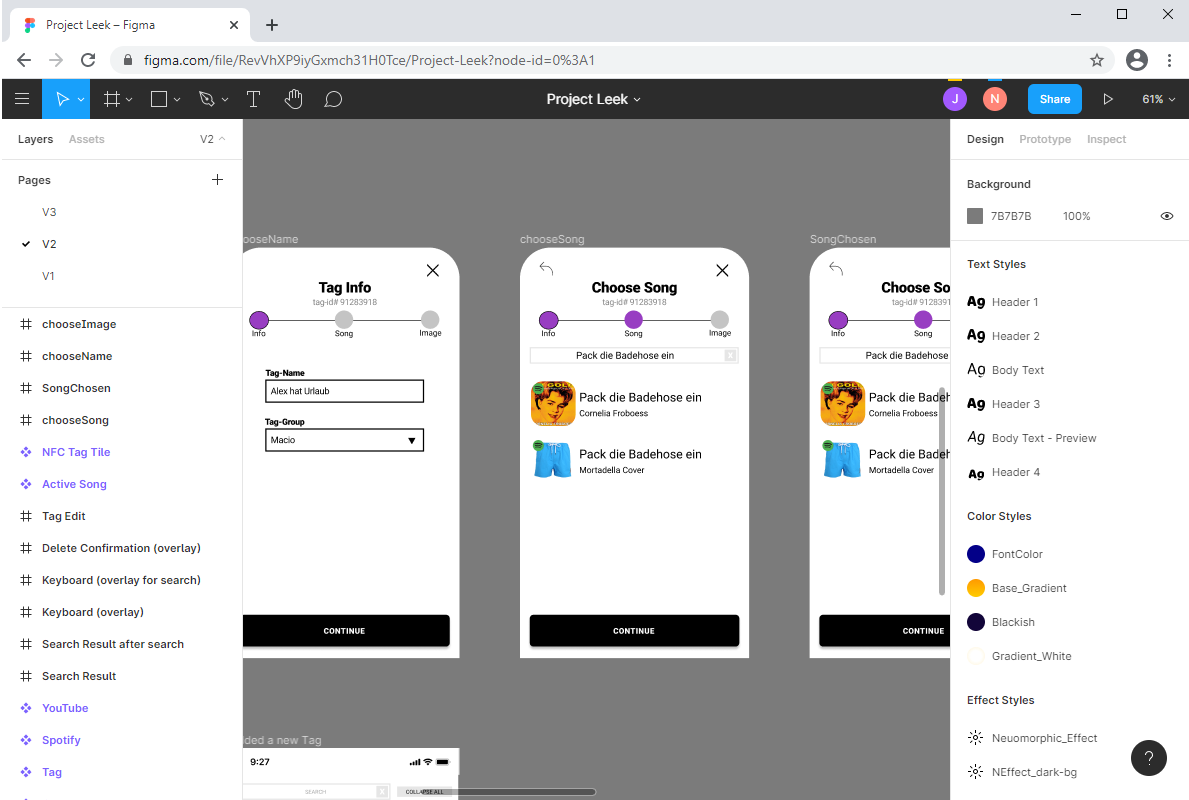
\includegraphics[width=8cm]{Figma.png}}{Proto\-typisierung mit \textit{figma}}
      \subsubsection{Prototyping (Figma)}
      \label{figma}
      Zur Abstimmung auf ein Design für die Benutzer\-oberfläche wurden vor der Entwicklung Proto\-typen der benötigten Komponenten mittels des webbasierten
      Prototyping-Tools \textit{figma}\footnote{https://www.figma.com/} konzipiert. So konnten neben dem Design auch Abläufe in Form von \glqq Click-Dummys\grqq{} erstellt werden und mit dem Kunden abgestimmt werden.
      \textit{Figma} wurde verwendet, da es einen kollaborativen Zugriff ermöglicht, kostenlos ist und bereits Erfahrung mit der Plattform bestand.

      \wrapfiguresafe{r}{0mm}{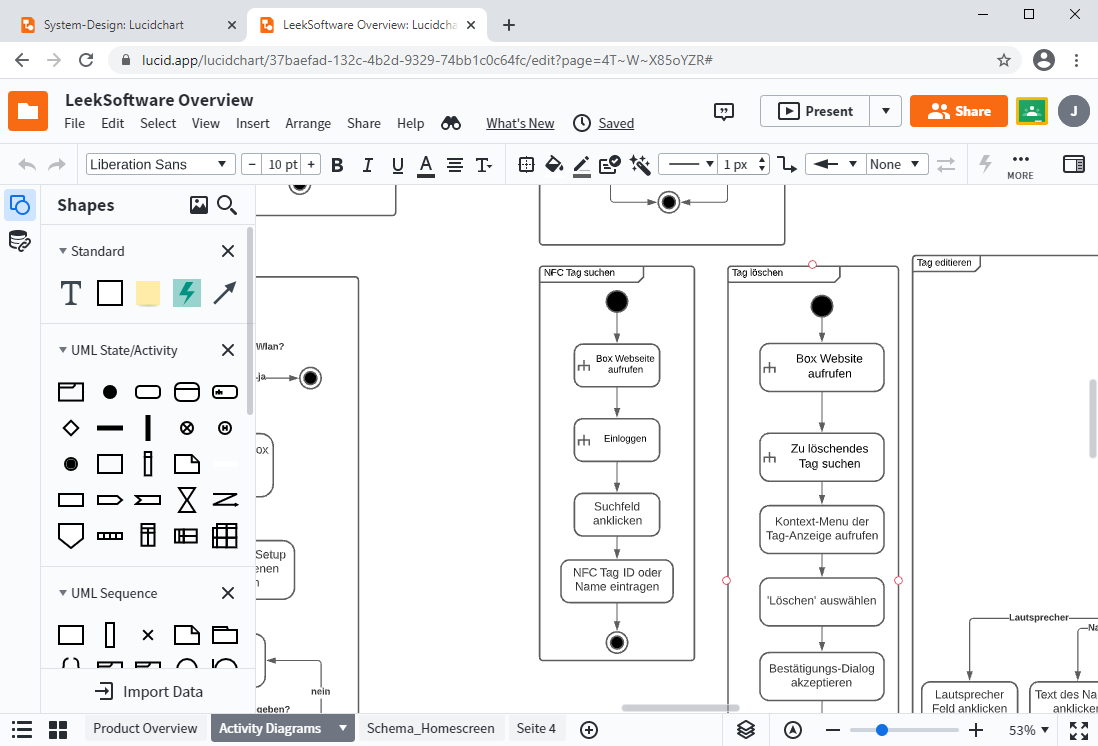
\includegraphics[width=8cm]{Lucidchart.png}}{Zeichnen von Diagrammen mit \textit{Lucidchart}}
      \subsubsection{Lucidchart}
      \label{Lucidchart}
      Um Abläufe schon vor dem Prototyping skizziert darstellen zu können wurde außerdem die webbasierte Plattform \textit{Lucidchart}\footnote{\raggedright\url{https://www.lucidchart.com/}} verwendet.
      Hier wurde neben der initial erstellten Produktübersicht auch mehrere Aktivitätsdiagramme erstellt, die aus vom Projektteam entwickelten und mit dem Kunden abgestimmten User-Stories entstanden sind.
      Diese sind im Anhang unter \ref{anhang:lucidchart} zu finden.
      Auch diese Plattform ermöglicht den gleichzeitigen Zugriff und war den Entwicklern bereits bekannt, was die Notwendigkeit der Einarbeitung eliminierte.

  \subsection{Entwicklungszyklus}
    Während der Umsetzung der \textit{leek-box} durchlief jedes Teammitglied für jedes \textit{Issue} den am Anfang des Projekts festgelegten und
    durch die Retrospektiven optimierten Zyklus.
    \\~
    Am Anfag steht die Auswahl eines \textit{Issues} aus der Spalte \textit{ToDo} des \textit{Issue Boards}.
    Nach Identifikation weist sich der Entwickelnde dem Ticket zu. Daraufhin erstellt der verwendete Bot automatisch einen \textit{Branch}
    in dem Schema \textit{[Ticket\-nummer]-[Ticketname]}. Nun kann mit der Arbeit in \textit{Visual Studio Code} begonnen werden.
    \\~
    \wrapfiguresafe{r}{0mm}{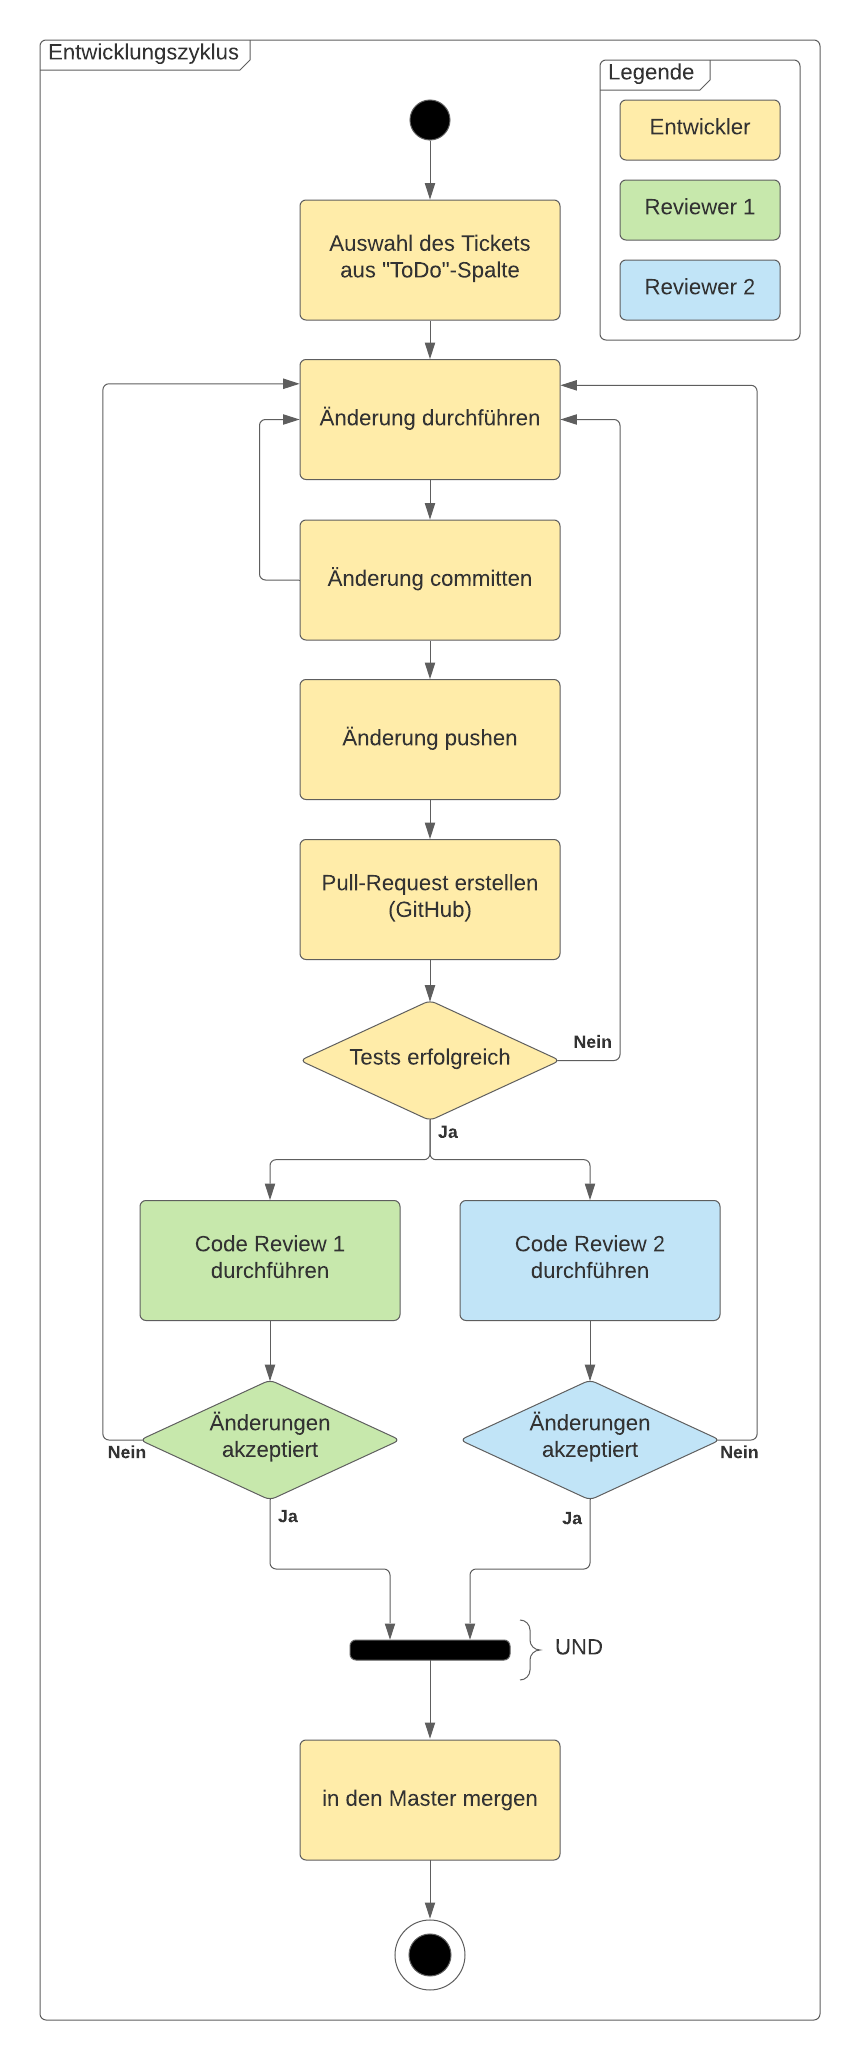
\includegraphics[width=0.62\textwidth]{Entwicklungszyklus.png}}{Entwicklungszyklus}
    Die Änderungen sollten möglichst kleinschrittig aber sinnvoll \textit{comittet} und anschließend \textit{gepusht} werden.
    GitHub erkennt automatisch die neuen \textit{commits} und erfragt, ob ein neuer \textit{Pull-Request} angelegt werden soll.
    Dieser hat initial den Status \textit{Open}.
    Wenn die Aufgaben des \textit{Issues} noch nicht abgeschlossen sind, wird der Status auf \textit{Draft} gesetzt.
    \\~
    Nach dem \textit{push} aller Änderungen, wird das Ergebnis der automatisierten Tests (\textit{GitHub Actions}) ermittelt. Treten hierbei Fehler auf,
    werden diese geprüft und behoben. Sind alle Tests erfolgreich, betätigt der Entwickelnde die Schaltfläche \textit{Ready for Review}.
    Wenn ein:e Entwickler:in, diesen \textit{Pull-Request} sieht, wird ein \textit{Code-Review} durchgeführt.
    Hierzu wird der Branch in die IDE geladen und die Funktionalität verifiziert. Anschließend wird die Code-Qualität geprüft.
    Dafür werden die geänderten Dateien im Pull-Request betrachtet. Anmerkungen können in Form
    von Kommentaren an einzelne oder mehrere Zeilen angefügt werden. Bei Änderungsvorschlägen können diese über eine \textit{suggestion}
    getätigt werden. Ist der komplette Code geprüft wird entschieden,
    ob die Änderungen angenommen (\textit{approve}) werden oder eine Änderungsanforderung gestellt wird (\textit{Request changes}).
    \\~
    Im Falle von Änderungsanforderungen werden diese umgesetzt und ein erneutes Review angefordert. Dies geschiet zyklisch, bis die Änderungen angenommen werden.
    Sind die Änderungen durch zwei \textit{Code-Reivews} bestätigt worden, werden sie mit der Schaltfläche \textit{Mege into master} übertragen.

  \subsection{Testing}
  Das Team entschied sich zu Beginn der Produkt-Entwicklung dafür, Tests zur Verbesserung der Codequalität durchzuführen.
  Quellcode Tests lassen sich in statische und dynamische Tests unterteilen.

  \subsubsection*{Statische Tests}
    Im Allgemeinen untersuchen statische Tests nur Textdokumente und betrachten im Gegensatz zu dynamischen Tests nicht das Verhalten zur Laufzeit.
    Dies ermöglicht eine häufige und kontinuierliche Nutzung von Tests dieser Art.
    Zwei der prominenten Varianten statischer Tests, Linting und Reviews, wurden in diesem Projekt genutzt.

    \paragraph*{Linting}$~$ \\
    Beim Linting wird der Code auf syntaktische Korrektheit geprüft.
    Auch manche semantische (laufzeitunabhängige) Aspekte werden untersucht.
    So können kleinere Denkfehler und Flüchtigkeitsfehler, wie z. B. fehlende Kommata, schnell gefunden und behoben werden.
    Hierfür wurde das Analyse-Werkzeug \textit{ESLint}\footnote{\raggedright\url{https://eslint.org/}} genutzt.
    Für diese Werkzeug war zusätzlich auch eine Erweiterung\footnote{\raggedright\url{https://marketplace.visualstudio.com/items?itemName=dbaeumer.vscode-eslint}} für die Entwicklungsumgebung verfügbar.
    Mit dieser konnten die Ergebnisse des Linting direkt im Code angezeigt werden.
    Dies machte den Arbeitsprozess wesentlich zeiteffizienter.
    Zusätzlich wurde auch die Erweiterung \textit{Vetur}\footnote{\raggedright\url{https://vuejs.github.io/vetur/}} genutzt.
    Diese stellte die selben Funktionalitäten für den Vue-Framework spezifischen Code zur Verfügung.
    \\
    Darüber hinaus boten diese Erweiterungen auch Formatierungshilfen mit übertragbaren Konfigurationen, durch deren Nutzung ein konsistenter Code-Stil
    innerhalb des Teams ermöglicht wurde. Dies legte den Grundstein für lesbaren Code und ermöglichte successive effizientes Arbeiten.

    \paragraph*{Reviews}$~$ \\
    Teil des Deployment Cycles waren auch Reviews der aktiven Änderungen.
    Bei diesen wurde der neue bzw. geänderte Quellcode von mindestens zwei anderen Teammitgliedern überprüft.
    Untersucht wurden vor allem semantische Fehler, Lesbarkeit, Wartbarkeit und Vollständigkeit.
    Hierfür gab es keinen formalen Plan, allerdings war die Review-Oberfläche von GitHub sehr hilfreich.
    In dieser wurde eine Änderungsansicht (\textit{diff}) des zu überprüfenden Codes angezeigt, auf der alle Teile des neuen Codes auf einen Blick einsehbar waren.
    Darüber hinaus bot die Review-Oberfläche auch die Möglichkeit, direkt im Code einzelne oder mehrere Zeilen zu kommentieren.
    So konnten auch Änderungsvorschläge gemacht und direkt übernommen werden, war für einen effizienten Review-Prozess sorgte.

  \subsubsection*{Dynamische Tests}
    Als dynamische Tests wurden in diesem Projekt Anwendungsfall-basierte Tests genutzt.
    Bei diesen Testfällen werden User-Stories Schritt für Schritt \glqq durchgespielt\grqq{} und dabei überprüft, ob das Resultat  dem erwarteten Verhalten entspricht.
    Die meisten Test dieser Art wurden als Integrations-Tests durchgeführt, bei denen die Änderungen im Kontext der bestehenden Software getestet wurden.
    So konnte vor allem das Zusammenspiel von Frontend und NFC-reader mit dem Backend gut überprüft werden.
    Aufgrund der Komplexität dieser Kontrollen wurden diese manuell durchgeführt und nicht automatisiert.
    Die testenden Entwickler durchliefen bei der Überprüfung folgende Schritte:
    \begin{enumerate}
      \item Zu überprüfenden \textit{feature-branch} auschecken
      \item Projekt bauen und ausführen
      \item Neue oder geänderte Funktionen mit beispielhaften Eingaben nutzen (z.B. neue NFC-Tags anlegen)
      \item Gegebenenfalls Probleme und Fehler aufzeichnen und beheben
    \end{enumerate}
    Diese Tests waren Teil des Deployment Cycles und wurden so in den meisten Fällen parallel zu den Reviews durchgeführt.
    \\~\\
    Ein gewisser Teil der anwendungsfallbasierten Test fand auf der Ebene von Code-Funktionen (\textit{Units}) statt, welche zur einfacheren Wiederholbarkeit automatisiert wurden.
    Dazu wurde das JavaScript-Test-Framework \textit{Jest}\footnote{\raggedright\url{https://jestjs.io/}} genutzt, da sich Tests hiermit sehr intuitiv und ohne großen Lernaufwand schreiben ließen.
    Auch diese Tests waren Teil des Deployment Cycles und wurden so bei jedem Pull-Request automatisch ausgeführt.


\wrapfiguresafe{r}{0mm}{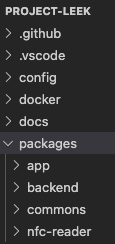
\includegraphics[width=4cm]{PackageStruktur.png}}{Orderstruktur}
\section{Technische Umsetzung}
  \subsection{Projektstrukur}
  \label{Ordnerstruktur}
  Die an das Projekt gesetzten Anforderungen machten die Erstellung mehrerer Applikationen notwendig. Neben einer Benutzeroberfläche, auf der die NFC-Tags
  verwaltet werden können, musste die Steuerung des NFC-Readers und ein System zur Speicherung der Daten sowie zum Abspielen der Musik entwickelt werden.
  Die dafür benötigten Anwendungen wurden als Microservices konzipiert und umgesetzt.
  Microservices sind kleine, separat ausführbare und eigenständige Dienste mit geringem Umfang.
  Diese kommunizieren untereinander mit allgemein verwendeten Protokollen, wie zum Beispiel HTTP, via APIs.
  Größere Projekte werden bei einer Mikroservice-Architektur dementsprechend in kleine Teile \glqq zerlegt\grqq ,
   die eigenständig entwickelt und betrieben werden können. \cite{Microservices}\\
  Zur Verringerung des Aufwands der Konfiguration, des Abhängigkeiten-Managements und der Wartung entschied sich das Team, die einzelnen Microservices auf GitHub in einem Repository zusammenzufassen. \cite{Monorepo}
  Repositories dieser Art werden \textit{mono-repositories} oder \textit{monorepos} genannt, da sich alle Komponenten an einem einzigen Ort befinden.
  Jeder Service wurde in einem Unterordner in \textit{packages} angelegt (vgl. Abbildung \ref*{Ordnerstruktur}). Der Ordner \textit{app} enthält die Benutzeroberfläche,
  \textit{backend} die Datenbankschnittstelle sowie Logik zur Kommunikation mit dem Musik-Streaming-Anbieter und \textit{nfc-reader} die Applikation zum Steuern und auslesen des am Raspberry Pi angeschlossenen NFC-Readers.
  Im Ordner \textit{commons} befinden sich von allen Services gemeinsam genutzte Ressourcen (wie z. B. Modell-Klassen).
  Neben den einzelnen Microservices wurden ebenfalls die Dokumentationsdateien wie Setup-Guide, Benutzerdokumentation und Projektbericht im Mono-Repo im Ordner \textit{docs} abgelegt.
  Auch die für den Dienst \textit{Docker} benötigten Dateien fanden in dem gleichnamigen Ordner Platz. Die Konfigurationsdateien für \textit{ESLint} und den \textit{Typescript}-Compiler sind im Ordner \textit{config} zu finden.
  Auf die Auflistung aller weiteren Dateien wird in diesem Bericht verzichtet. Eine genaue Aufstellung ist dem \textit{GitHub-Repository}\footnote{\url{https://github.com/project-leek/project-leek}} zu entnehmen.
  Durch die Zusammenfassung in ein Mono-Repository waren die einzelnen Services für jeden Entwickler jederzeit einfach erreichbar, ohne die Notwendigkeit das Repository zu wechseln.

  \begin{figure}[h]
    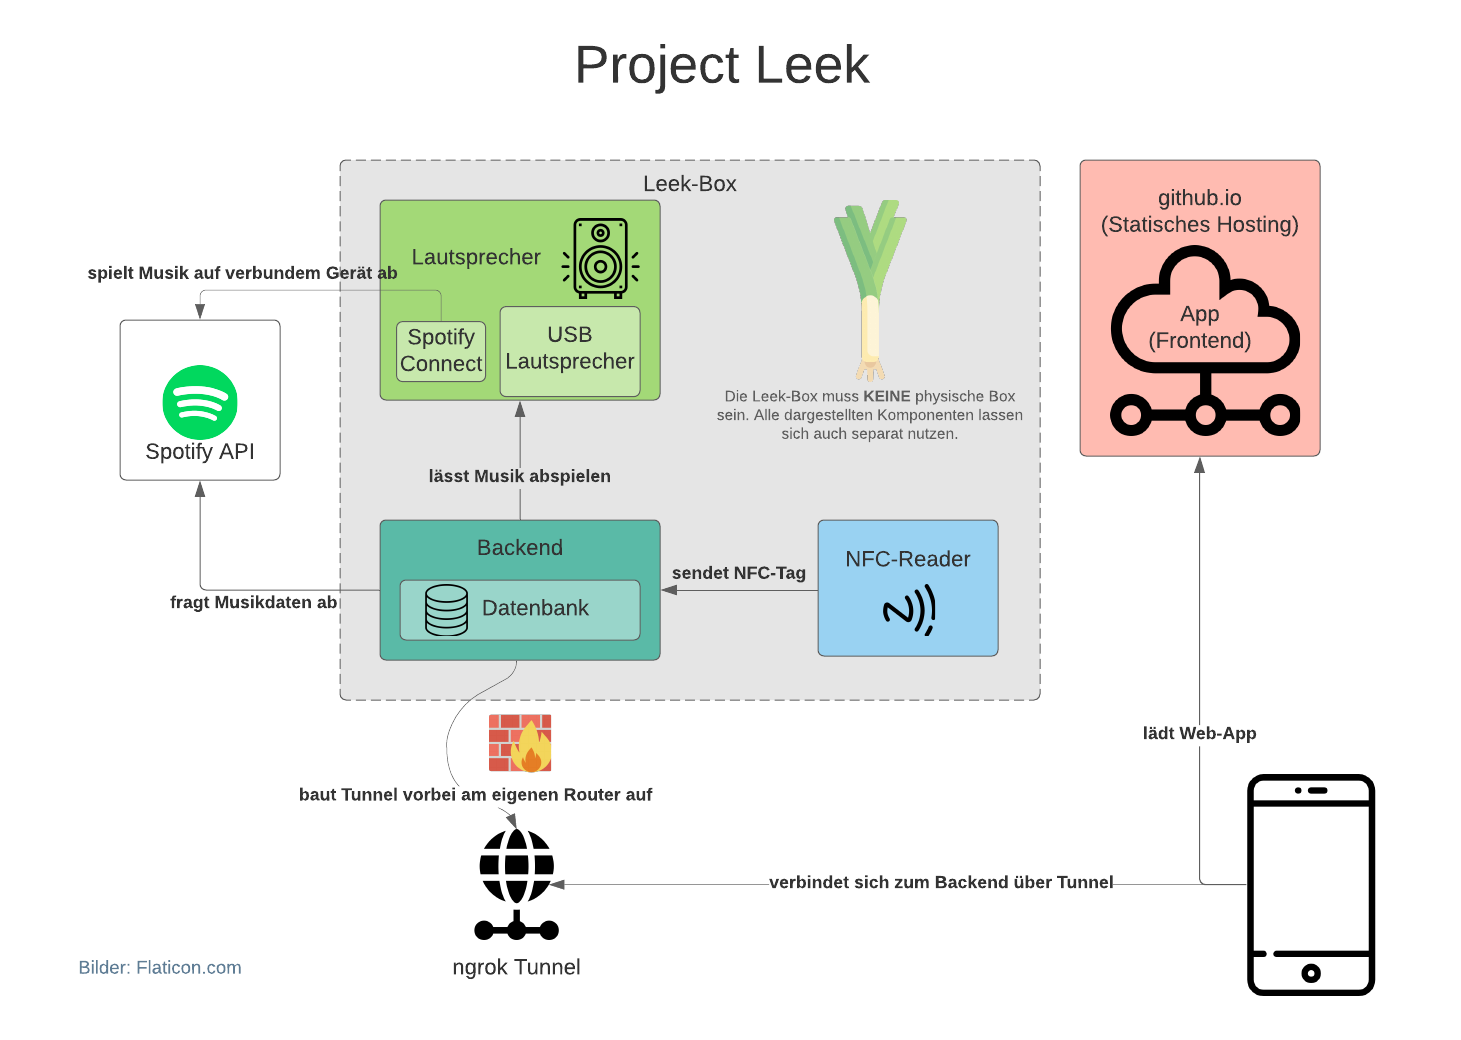
\includegraphics[width=\linewidth]{LeekSoftware_Overview.png}
    \caption{Überblick zum Aufbau der Leek-Software}
    \label{fig:LeekSoftwareOverview}
  \end{figure}

  \subsection{Technologien}

  \label{technologien}

  \subsubsection{Programmiersprachen}

  \paragraph*{TypeScript} $~$ \\
  Da alle Teammitglieder bereits Erfahrungen mit JavaScript gesammelt hatten wurde diese zuerst als Programmiersprache vorgeschlagen.
  Aufgrund von nicht vorhandener Typisierung wurde sich dann jedoch auf die von Microsoft entwickelte Sprache TypeScript geeinigt. Diese bietet aufgrund des
  Aufbaus auf den ECMAScript-6-Standards eine große syntaktische Ähnlichkeit zu JavaScript. Somit fiel das Erlernen der Sprache den Entwicklern relativ leicht.
  Durch die starke Typisierung entstehen außerdem weniger Laufzeitfehler, da die entwickelnde Person bereits zur Compile-Zeit auf Typfehler aufmerksam gemacht wird.\cite{Typescript_Typisierung}
  Bei der Kompilierung von TypeScript-Code wird dieser zu gültigem JavaScript Code umgewandelt, wodurch auf eine Vielzahl von bereits existierenden JavaScript-Paketen zugegriffen werden konnte.
  Außerdem lässt sich Typescript durch Nutzung der Laufzeitumgebung Node.js auch als Backendsprache verwenden und ersparte dem Team damit die Nutzung von verschiedenen Programmiersprachen.


  \subsubsection{Frameworks}
  Neben der Programmiersprache Typescript setzte das Team verschiedene Frameworks ein, um mit weniger Aufwand entwickeln zu können.

  \paragraph*{Vue.js} $~$ \\
  Zur Gestaltung der Benutzeroberfläche für die \textit{leek-box}, die zum Verwalten der NFC-Tags und Steuern der Ausgabegeräte genutzt wird, einigte sich das Team auf die Nutzung des
  clientseitigen JavaScript-Webframeworks \textit{Vue.js}\footnote{\raggedright\url{https://vuejs.org/}}
  Dieses wurde vor allem aufgrund dessen Haupteigenschaften \textit{components} und \textit{reactivity} entschieden.

  \paragraph*{Components} $~$ \\
  Durch Vue lassen sich Webseiten mit HTML, CSS und JavaScript bzw. TypeScript erstellen. Dabei bietet das Framework, im Vergleich zur Webentwicklung ohne Framework, die Möglichkeit sogenannte Single-File-Components (\textit{.vue} Dateien) zu nutzen. In diesen können sich ein Template für das HTML-Grundgerüst, ein Bereich für CSS Styles und die Logik der Komponente, welche aus JavaScript oder TypeScript Code besteht, befinden. Dies ermöglicht eine inhaltiche Zusammenfassung aller Teilaspekte eines Elementes der Webseite in einer einzigen Datei.
  \\~\\
  \begin{minipage}{\textwidth}
    \begin{lstlisting}[caption={Beispiel einer simplen \textit{vue component}-Datei}, captionpos=b, label=lst:EinfacheComponent]
      <template>
        <span class="beispiel">Beispiel Komponente</span>
      </template>

      <script lang="ts">
      import { defineComponent } from 'vue';

      export default defineComponent({
        name: 'Beispiel',
      });
      </script>
      <style>
        .beispiel {
          background-color: lightgreen;
        }
      </style>
    \end{lstlisting}
  \end{minipage}

  Durch diese Zusammenfassung wird der gesamte Code lesbarer,
  da meist nur eine Datei je gerade behandeltem Element des Frontends konsultiert werden muss.
  So wird Entwickleren viel Suchzeit und Arbeitsaufwand gespart werden, die anderweitig angefallen wären.
  Dies führte zu effizienterem und zufriedenstellenderer Arbeit am Projekt.
  Bessere Lesbarkeit führt auch zu langfristigerer Wartbarkeit.
  Dies ist in diesem Projekt besonders wichtig,
  da es unter Open-Source-Lizenz steht und gegebenenfalls von der Allgemeinheit weiter entwickelt werden soll.
  Mit adäquater Wartbarkeit ist eine Grundlage für langjähriges Überleben der \textit{leek-box} geschaffen.
  \\~\\
  Ausmaß, Funktionalität und Größe von Komponenten sind allgemein keine Einschränkungen gesetzt.
  So kann es sich bei diesen zum Beispiel um Buttons, Header oder ganze Ansichten handeln.
  Für die Nutzung müssen diese allerdings noch mit \textit{defineComponent} beim Framework registriert werden
  (siehe Listing \ref{lst:EinfacheComponent}).
  Danach können die Komponenten wie native HTML-Tags eingebunden werden.
  Dies macht die Nutzung von \textit{components} sehr intuitiv.
  So hat das Framework eine sehr flache Lernkurve.
  Die Verwendung von weitreichend klassischem HTML, CSS und JS bzw. TS unterstützt dies zusätzlich.
  Für das Team war dies immens wertvoll und ein wichtiges Auswahlkriterium für die Wahl der Technologien,
  da für das Projekt nur wenige Monate Zeit zur Verfügung standen.
  \\~\\
  \textit{Components} können auch innerhalb von anderen \textit{components} genutzt werden.
  So lassen sich komplexere Elemente des Frontends aus kleineren, übersichtlicheren Komponenten zusammensetzten.
  Um dies zu ermöglichen, können von der aufrufenden Instanz Daten an die Komponenten übergeben werden.
  Anhand dieser können Inhalte, Aussehen und Verhalten dem Kontext entsprechend angepasst werden.
  Die Datenübergabe wird über sogenannte \textit{properties} (kurz \textit{props}) realisiert.
  Auch der Informationsfluss in die andere Richtung ist möglich und geschieht über \textit{events}, welche von eingebundenen Komponenten erzeugt und ausgelöst werden können.
  Dabei ist es möglich Daten als Argumente an die \textit{events} anzuhängen, damit die einbindende Komponente diese dann auslesen und weiterverwenden kann.
  Dies wird folgend in Listing \ref{lst:Liste} und \ref{lst:Eintrag} dargestellt.
  \\~\\
  \begin{minipage}{\textwidth}
    \begin{lstlisting}[caption={beispielhafte Listen-Komponente (Liste.vue)}, captionpos=b, label=lst:Liste]
      <template>
        <eintrag v-bind:name="'eins'" @eintrag-geklickt="geklickt($event)" />
        <eintrag v-bind:name="'zwei'" @eintrag-geklickt="geklickt($event)" />
        <eintrag v-bind:name="'drei'" @eintrag-geklickt="geklickt($event)" />
      </template>

      <script lang="ts">
      import { defineComponent } from 'vue';

      import Eintrag from './Eintrag.vue';

      export default defineComponent({
        name: 'Liste',
        components: {
          Eintrag,
        },
        setup() {
          function geklickt(wert: string): void {
            console.log(wert);
          }
          return { geklickt };
        },
      });
      </script>
    \end{lstlisting}
  \end{minipage}

  \begin{minipage}{\textwidth}
    \begin{lstlisting}[caption={beispielhafte Eintrag-Komponente (Eintrag.vue)}, captionpos=b, label=lst:Eintrag]
      <template>
        <button @click="$emit('eintrag-geklickt', rückgabe)">{{ name }}</button>
      </template>

      <script lang="ts">
      import { defineComponent } from 'vue';

      export default defineComponent({
        name: 'Eintrag',
        props: {
          name: {
            type: String,
            default: 'Name',
          },
        },
        emits: ['eintrag-geklickt'],
        setup(props) {
          const rückgabe: string = 'Eintrag ' + props.name + ' ausgewählt';
          return { rückgabe };
        },
      });
      </script>
    \end{lstlisting}
  \end{minipage}

  Hierbei gibt die Listen-Komponente die entsprechenden Namen an die \textit{Eintrag}-Komponenten
  mit dem prop \glqq name\grqq{} per \textit{v-bind:} an die Einträge weiter.
  Die verwendete \textit{property} \glqq name\grqq{} wird in dem Eintragselement angezeigt und beim Klicken auf dieses mit einem Event per \textit{\$emit} an die Eltern-Komponente \textit{Liste} zurückgesendet. Der mitgelieferte Wert des Events wird mit \textit{\$event} ausgelesen und zur Veranschaulichung in der Konsole ausgegeben.
  \\~\\
  Alles in allem ermöglichte die Verwendung von \textit{components} dem Team die Produktion von schlankem und übersichtlichen Frontend-Code.

  \paragraph*{Reactivity}$~$ \\
  Reaktive Programmierung ist ein Programmierparadigma, welches Abstraktionen bereitstellt,
  um Werte, die sich nachträglich ändern können, zu nutzen
  und Abhängigkeiten zwischen diesen Werten abzubilden. \cite{ReactiveProgramming}
  Als Paradebeispiel hierfür werden meist Tabellenkalkulationswerkzeuge wie zum Beispiel \textit{Excel} angeführt.
  In diesen lassen sich Rechenergebnisse von den momentanen Werten anderer genutzter Zellen abhängig machen.
  Entsprechend ändert sich auch das Ergebnis automatisch, wenn Eingabewerte geändert werden. \\
  Auch \textit{Vue} ermöglicht es, diese Art von Funktionalität einzusetzten.
  So können reaktive generische Datentypen z. B. in components verwendet werden.
  In diesem Projekt wurden dafür vor allem \textit{reactive} für Objekte und \textit{ref}
    \footnote{\raggedright\url{https://v3.vuejs.org/guide/reactivity-fundamentals.html}} für primitive Datentypen verwendet.
  Wie das Beispiel in Listing \ref{lst:reactivity} demonstriert, können so Datenänderungen sehr einfach angezeigt werden, da eine Referenz an Stelle einer eigentlichen Instanz übergeben wird, welche sich somit automatisch aktualisiert.
  \\~\\
  \begin{minipage}{\textwidth}
    \begin{lstlisting}[caption={Demonstration reaktivier Vue-Referenzen}, captionpos=b, label=lst:reactivity]
      <template>
      <div>
        <span>{{ count }}</span>
        <button @click="count ++">Increment count</button>
      </div>
    </template>

    <script lang="ts">
      import { ref } from 'vue';
      export default defineComponent({
        setup() {
          const count = ref(0);
          return { count };
        },
      });
    </script>
    \end{lstlisting}
  \end{minipage}
  In diesem Beispiel wird bei Instanziierung der Komponente (in \textit{setup}) ein Zähler als reaktive Vue-Referenz (\textit{ref}) angelegt.
  Dieser wird bei jedem Klick auf den Button inkrementiert.
  Da dies im HTML-Code passiert, wird der Wert hinter der Referenz direkt manipuliert.
  Dagegen muss im TypeScript-Code der Wert vorher noch mit \textit{count.value++} \glqq ausgepackt\grqq{} werden.
  Der geänderte Wert wird direkt auf der Webseite angezeigt,
  ohne das diese neu geladen oder das DOM durch den Entwickler manipuliert werden muss. Stattdessen werden jeweils nur die grundlegenden Daten einer Komponente verändert und Vue bildet diese Daten mit Hilfe des Templates im DOM ab.
  \\
  Dieses Paradigma findet auch in der Kommunikation zwischen verschachtelten \textit{components} Anwendung.
  So sind alle \textit{properties} von Komponenten reaktiv. Auch die an Events angehängten Daten können reaktiv sein.
  Dies ermöglichte dem Team in kurzer Zeit interaktive Benutzeroberflächen zu erstellen.

  \paragraph*{}
  Ein weiterer, weniger zentraler Faktor für die Wahl des Frameworks \textit{vue} war die Performanz.
  Dies zeigt sich im Vergleich zu anderen Web-Frameworks in Benchmark-Tests.\cite{Vue_Performance}
  Für das Projekt war dies vor allem wichtig, da das System auf einem Raspberry Pi betrieben werden sollte
  und dementsprechend nur begrenzte Leistung zur Verfügung steht.

  \paragraph*{Tailwind CSS} $~$ \\
  Zur effizienteren Gestaltung der Benutzeroberfläche entschied sich das Team für das Utility-First-Framework \textit{TailwindCSS}\footnote{\raggedright\url{https://tailwindcss.com}}.
  Dieses bietet im Vergleich zu anderen CSS-Frameworks wie \textit{Bootstrap} mehr Flexibilität, da statt vorgefertigten Komponenten vielseitig verwendbare Utility-Klassen zur Verfügung gestellt werden,
  über die das Design definiert werden kann. So kann das Aussehen von Elementen innerhalb des HTML-Codes festgelegt werden.
  Damit steigt die Übersichtlichkeit des Frontend-Codes, da keine separaten CSS-Dateien und -Klassen angelegt werden müssen.
  \cite{Tailwind_Vorteile}


  \paragraph*{FeathersJS} $~$ \\
  Bei der Erstellung des Backends entschied sich das Team zusätzlich das Framework \textit{FeathersJS}\footnote{\raggedright\url{https://feathersjs.com/}} einzusetzten.
  Dies ermöglicht komfortable CRUD-Zugriffe\footnote{CRUD = \textbf{C}reate-\textbf{R}ead-\textbf{U}pdate-\textbf{D}elete}  auf verschiedene Services, welche zum Beispiel Datenbanken oder externe APIs sein können.
  Durch eine vielzahl von Adapatern können so zum Beispiel Daten in einer Datenbank ohne eigene Implementierung der Schnittstelle verwaltet werden.
  Es muss lediglich ein Service erstellt werden, der das generische Interface Service mit Typeparameter der zu verwaltenden Klasse implementiert. (vgl. Abb. \ref{fig:MyService})
  \begin{figure}[ht]
    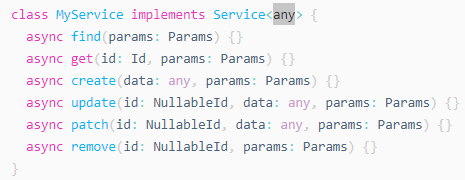
\includegraphics[width=\linewidth]{MyFeathersService.png}
    \setcaptioncitation{https://docs.feathersjs.com/guides/basics/services.html}
    \caption{Implementierung eines ServicesTest}
    \label{fig:MyService}
  \end{figure}
  Dabei können verschiedenste Protokolle, wie HTTP oder WebSockets zur Datenübertragung verwendet werden.
  Das WebSocket-Protokoll bietet hier den großen Vorteil, dass eine persistente Verbindung zwischen Server und Client (Benutzeroberfläche und Backend) besteht.
  So können sowohl Client, wie auch Server jederzeit mit der Datenübertragung beginnen, ohne vorher - wie bei HTTP - jedes Mal eine neue Verbindung aufzubauen zu müssen. \cite{WebSockets}
  Dadurch kann der Server alle verbundenen Clients bei einem CRUD-Zugriff informieren, sodass alle ohne erneutes Anfragen der Daten den aktuellsten Zustand übermittelt bekommen.
  Wird also beispielsweise ein NFC-Tag von Person A geändert, sieht Person B diese Änderung ohne manuelle Aktualisierung der Seite.
  Eine weiteres Feature, welches vom Projektteam genutzt wurde ist die integrierte OAuth-Provider-Abstraktionen, die ein einfaches Authentifizieren mit Diensten, wie beispielsweise \textit{Spotify} bei diesem Projekt ermöglicht.
  Dies war z.B. nötig, um die den NFC-Tags zugeordnete Musik abspielen zu können.
  Darüber hinaus können so auch Nutzerprofile angelegt werden, ohne persönliche Daten, wie z.B. Namen, Email-Adressen und Passwörter, speichern zu müssen.
  Nur Authentifizierungstokens des OAuth-Providers werden in der Datenbank hinterlegt.
  So konnte ein besserer Datenschutz für die Nutzenden ermöglicht werden.


  \subsubsection{Containervirtualisierung (Docker)}
  Es wurde lediglich die Anforderung gestellt, dass die Applikation vor allem für mobile Endgeräte optimiert sein soll.
  Auf Basis dieser Anforderung evaluierte das Projektteam bekannte Technologien und recherchierte mögliche Alternativen.
  Um die Installation der Box möglichst komfortabel zu gestalten, wird auf die freie Containervirtualisierungssoftware \textit{Docker}\footnote{https://www.docker.com/} gesetzt.
  Ohne diese Möglichkeit wäre die Installation aufgrund der drei Microservices (Backend, Reverse-Tunnel und NFC-Reader) sehr aufwändig.
  Der Vorteil von Docker besteht darin, dass das Team lediglich eine sogenannte \textit{docker-compose} Datei benötigt, in dem die Konfiguration der Docker-Container beschrieben ist.
  Es enthält einen Verweis auf die jeweiligen Container-Images, auf denen die Container aufbauen (z. B. leek-backend). Diese Images enthalten bereits alle notwendigen Abhängigkeiten und Programme,
  sodass weitere Installationen seitens der Benutzer:innen nicht erforderlich sind.
  Außerdem lässt sich das Verhalten der Images durch Umgebungsvariablen weiter konfigurieren. Durch die einfache Auslieferung bietet Docker außerdem den Vorteil der Reproduzierbarkeit.
  So können aufgetretene Fehler problemlos von einem Entwickler nachgestellt werden, da Docker das Betriebssystem des Anwenders von der benötigen Umgebung der leek-box abstrahiert.


  \subsubsection{Reverse-Tunnel (ngrok)}
  \label{kapitel:ngrok}
  Um verschlüsselt vom Frontend (unter \raggedright\url{https://project-leek.github.io} erreichbar) auf das jeweilige Backend einer \textit{leek-box} zuzugreifen, wird der Reverse-Tunnel Dienst \textit{ngrok}\footnote{\raggedright\url{https://ngrok.com/}} verwendet.
  Dies ist notwendig, da moderne Browser eine verschlüsselte Verbindung (mit SSL-Zertifikat) zu allen Komponenten auf der Website verlangen, sobald die Website selbst per SSL geladen wird.
  Da das Framework jedoch nativ kein HTTPS unterstützt, wird \textit{ngrok} verwendet, um die unverschlüsselten Daten durch einen verschlüsselten Tunnel zum Frontend zu schicken. Damit wird die Anforderung der Verschlüsselten Verbindung erfüllt.
  Außerdem soll das Backend unabhängig vom lokalen Netzwerk erreichbar sein, ohne dass eine umständliche Portweiterleitung eingerichtet werden muss. Um dies zu leisten, baut das Backend einen Tunnel zu dem Server mit der bekannten Adresse \url{ngrok.io} auf.
  Dabei wird eine zufällige Subdomain im Schema \textit{xyz.ngrok.io} angelegt und dem Benutzer in der Konsole des Backends angezeigt. Diese Adresse kann der Benutzer nun im Frontend (\url{https://project-leek.github.io}) eingeben, um sich mit seiner Box zu verbinden.
  \colorbox{red}{Hier Schaubild?}

  \subsubsection{Externe Bibliotheken}
  \paragraph{Spotify Web API} $~$ \\
  \label{SpotifyWebApiNode}
  Um die abspielbaren Songs inklusive Cover-Bildern zu ermitteln und diese abzuspielen ist ein Zugriff auf die API eines Musikstreaming-Dienstes notwendig.
  Der vom Kunden vorgeschlagene Anbieter war \textit{Spotify}\footnote{\url{https://www.spotify.com}}.
  Um den Zugriff auf die Spotify API zu simplifizieren wurde die Bibliothek \textit{Spotify Web API Node}\footnote{\url{https://github.com/thelinmichael/spotify-web-api-node}} verwendet.
  Diese bietet bereits die benötigten Methoden, wie z. B. die zum Suchen eines Songs anhand eines Suchbegriffs.
  Neben dem Songtitel und der Spotify-Url werden auch die Künstler und die Adresse des Albumcovers mitgeliefert und konnten von den Entwicklern ohne Mehraufwand genutzt werden.
  Auch eine Methode zur Ermittlung der verfügbaren Geräte zum Abspielen der Musik stellt die Bibliothek bereit.

  \paragraph{NeDB} $~$ \\
  Als Datenbank für dieses Projekt wurde die kostenlos verfügbare JavaScript-Datenbank \textit{NeDB}\footnote{\raggedright\url{https://github.com/louischatriot/nedb}} gewählt.
  Sie wird verwendet, um die NFC-Tags, Benutzer und den angeschlossenen NFC-Reader zu verwalten.
  \textit{NeDB} ist eine auf \textit{MongoDB}\footnote{\raggedright\url{https://www.mongodb.com/}} aufbauende, sehr schnelle JSON Datenbank.
  Sie wurde gewählt, da sie eine geringe Komplexität besitzt und weil \textit{FeathersJS} einen Datenbankadapter für diese Datenbank bereitstellt, was den Zugriff auf die Datenbank sowie die Verwaltung der Daten erleichterte.
  Außerdem arbeitet die Datenbank inkrementell, was das Risiko auf sehr große Datenbankdateien minimiert.
  Diese Eigenschaft war hilfreich, um die Datenbank auf einem Raspberry Pi betreiben zu können.
  Zu Beginn des Projekts diskutierte das Team die Technologien, mit denen die \textit{leek-box} umgesetzt werden sollte.
  Der Kunde ließ dem Projektteam hierbei sehr viele Freiheiten.

  \subsection{Hardware}
  \subsubsection*{Raspberry Pi}
  \wrapfiguresafe{r}{0mm}{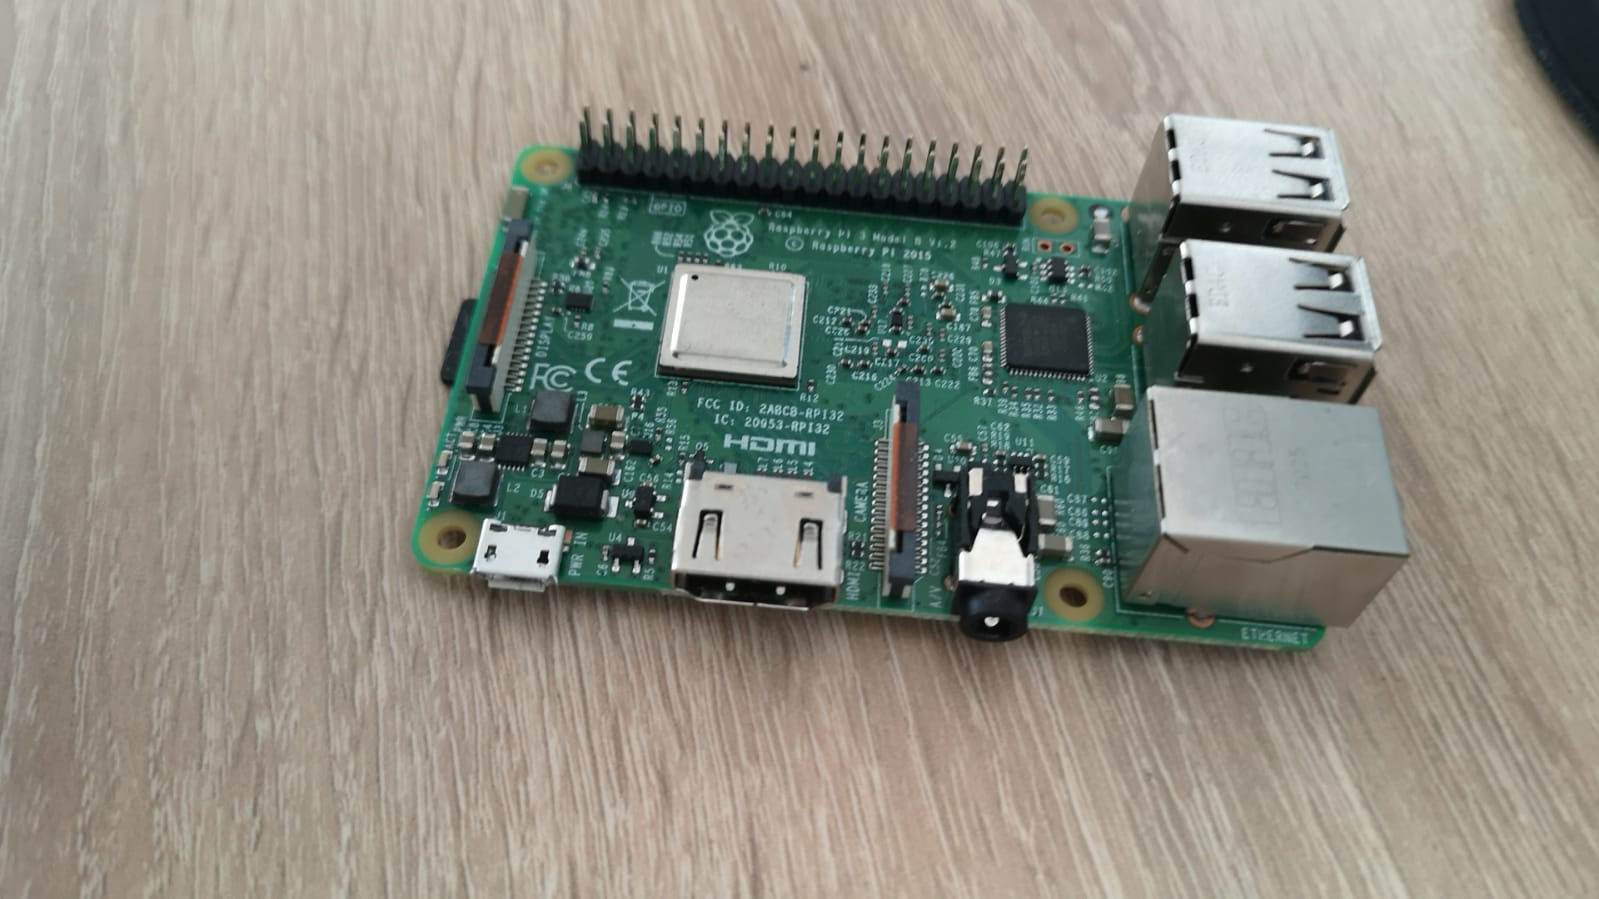
\includegraphics[width=0.45\textwidth]{RaspPi.jpeg}}{Raspberry Pi}
    Der Raspberry Pi ist ein Einplatinencomputer, welcher ein Ein-Chip-Systen (SoC) mit einer ARM-CPU enthält.
    Durch das gute Preis-Leistungsverhältnis, die einfache Programmierbarkeit und der sehr guten Verfügbarkeit sind Raspberry Pis sehr beliebt und haben sich für dieses Projekt als Hardwarewahl durchgesetzt.
    Hierbei fungierte der Pi für das Hosting des Backends sowie der Anbindung an einen NFC-Reader.

  \subsubsection*{NFC Tags \& NFC Reader}
  \wrapfiguresafe{r}{0mm}{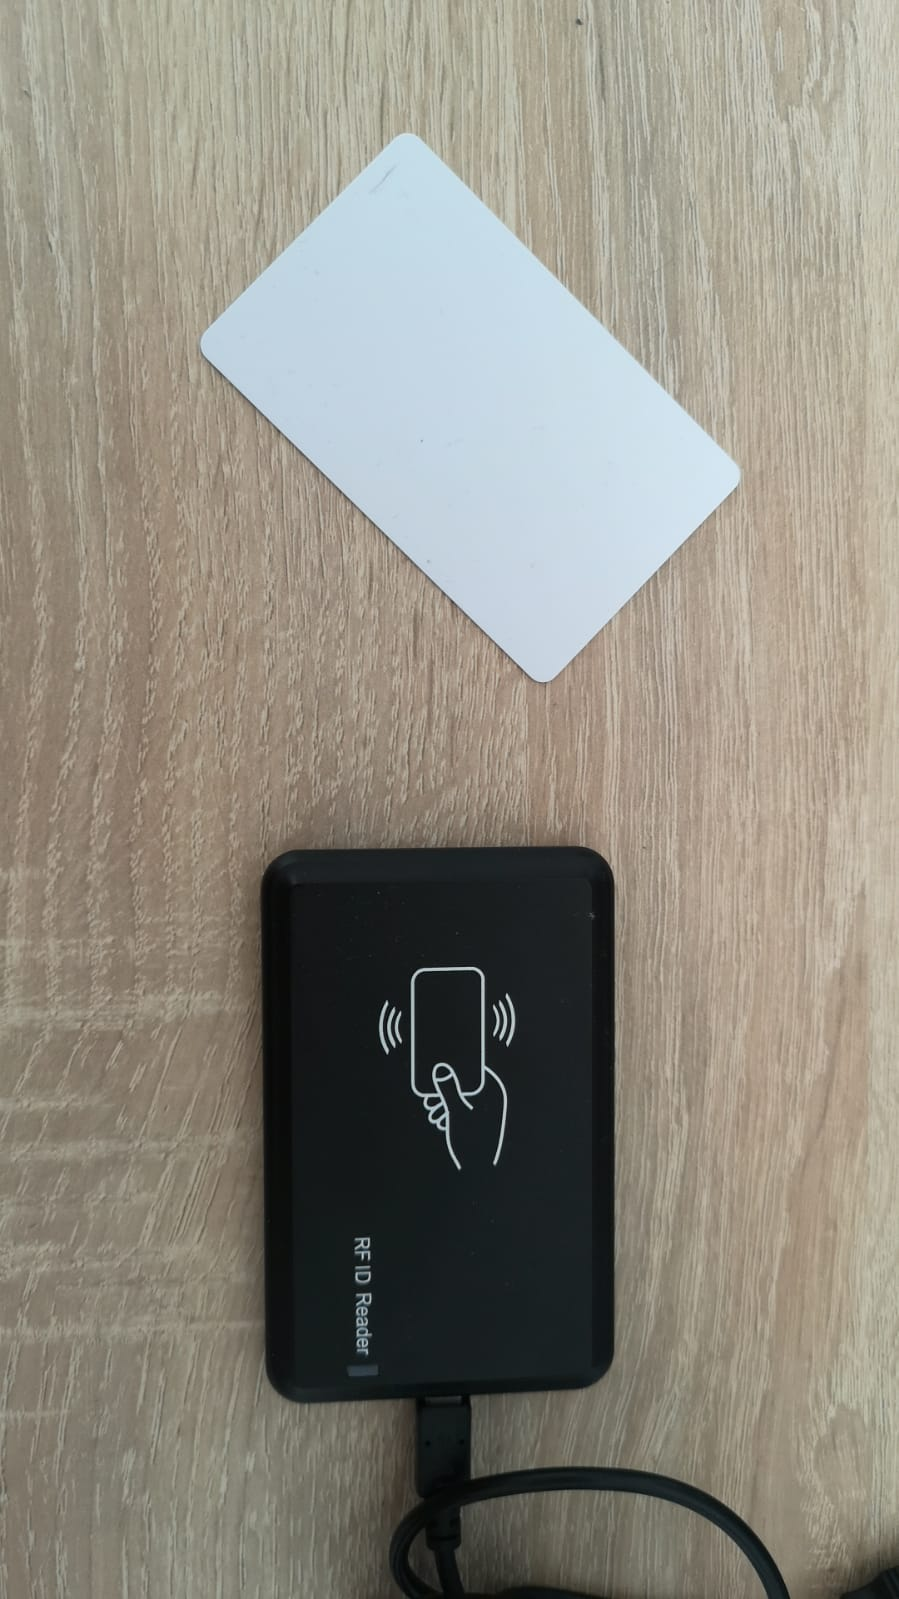
\includegraphics[width=0.25\textwidth]{NfcReaderAndTag.jpeg}}{NFC Reader und NFC Tag}
    Ähnlich wie bei Konkurrenzprodukten, wird als Peripheriegerät für den Raspberry Pi ein NFC Reader genutzt.
    Die Steuerung der Box kann so mittels NFC-Tags durchgeführt werden.
    NFC steht für \glqq Near Field Communication\grqq{} (Nahfeld-Kommunikation), ein Standard, der
    Datenübertragung auf sehr kurzer Distanz ermöglicht.
    NFC-Tags sind kleine Chips, die von einem NFC Reader ausgelesen werden können. Die Daten können je nach
    NFC Chip, von nur einer simplen \textit{Id} bis hin zu beschreibbaren NFC Tags mit unterschiedlichsten Daten
    variieren. In diesem Projekt wurden die primitiveren NFC-Tags, welche nur eine ID speichern, verwendet.

  \section{Durchführung}
\subsection{Meilenstein 1}
Die Laufzeit des ersten Meilensteins erstreckte sich vom 29.10.2020 bis zum 11.11.2020 und war auf die Planung, Struktur und das Vorgehen des Projektes fokusiert.
%Ziel
Zum Ende des Meilensteins sollte die Struktur und das Grundgerüst für das Projekt fertiggestellt sein.
Hierfür sollte das Konzept der Software-Architektur sowie die genutzten Technologien (später Technologie-Stack genannt) auf Basis einer Anforderungsanalyse mit dem Kunden festgelegt werden.
Außerdem sollten die ersten Tickets in das Backlog eingetragen werden.
Auch musste das Projekt dahingehend geplant werden, dass jedem Teammitglied durchgehend zu bearbeitende Arbeitspakete zur Verfügung standen.
Um ein schnellen und reibungslosen Start für die Entwicklung zu gewährleisten, sollte das Repository entsprechend vorbereitet werden.
%Probleme
Das Team musste das Projekt so entsprechend planen, dass jedes Teammitglied durchgehend sinnvoll arbeiten konnte.
%Lösungen
Durch bereits vorhandene Erfahrung mit verschiedenen Technologie-Stacks und ähnlichen Problemen, wurde sich auf den Technologie-Stack geeinigt
Die verwendeten Technologien sind dem Abschnitt \ref{technologien} zu entnehmen.
Um für jedes Teammitglieds ein sinnvolles kontinuierliches Arbeiten zu gewährleisten, einigte sich das Team auf einen ständig gefüllten Ticket-Pool im Repository, sodass jederzeit selbstständig eine Aufgabe gefunden und bearbeitet werden konnte.
%Product Increment
Das Ergebnis des ersten Meilensteins bestand, abweichend von den späteren, nicht in einem Produkt Inkrement, sondern legte die Grundbausteine für die Entwicklung und das Teamwork.
Neben dem bereits erwähnten Technologie-Stack, wurde als Host für die Applikation ein Raspberry Pi gewählt.
Für die Entwicklung wurde ein Mono-Repository mit \textit{lerna}\footnote{https://lerna.js.org/} aufgesetzt, welches Front- und Backend zusammenfasste.
Durch die Anforderung der Veröffentlichung als Open Source Projekt wurde eine verständliche und hilfreiche Dokumentation nötig, die einem Benutzer die Installation und Verwendung der \textit{leek-box} aufzeigt.
So wurde dem Repository eine einleitende Readme und ein \glqq How to Contribute\grqq{} Guide hinzugefügt.
%Retrospektive
Nach dem ersten Meilenstein fand noch keine nennenswerte Retrospektive statt.

\subsection{Meilenstein 2}
Der zweite Meilenstein wurde für den Zeitraum vom 11.11.2020 bis zum 25.11.2020 angesetzt.
Ziel war es, die ersten Grundbausteine für das Projekt legen. Damit das Team ein generelles Verständnis des Technologie-Stacks entwickeln konnte,
sollte jedes Teammitglied eine \glqq Hello-World\grqq{} Übungsaufgabe absolvieren. Diese beinhaltete das Anlegen eines Feathers-Services für ein virtuelles
Haustier im Backend und die Darstellung im Frontend. Auch die Grundstruktur für den Bericht zu dem Projekt sollte in diesem Milestone erstellt werden,
um den Fortschritt, Probleme und Erkentnisse zeitnah dokumentieren zu können.
\\~\\
\paragraph*{Hello-World (Pet)} $~$ \\
\label{HelloWorld}
Zur Umsetzung setzten sich die Entwickler mit der Dokumentation von Feathers auseinander um einen
Überblick über die notwendigen Klassen und Konstrukte zu erhalten. Zuerst musste eine Klasse erstellt werden, in der der Aufbau des Haustierts modeliert
wurde. Sie beinhaltete Attribute wie \glqq Name\grqq{} oder \glqq Id\grqq. Auf dieser Basis wurde anschließend ein Feathers-Service in Form einer
Klasse erstellt. Diese implementierte das von \textit{Feathers} bereitgestellte generische Interface \textit{Service<T>}. Als Typparameter wurde hier
die zuvor erstellte Model-Klasse angegeben. Um z. B. Objekte der Klasse \textit{NicksPet} zu verwalten wurde folgender Service angelegt:
\\~\\
\begin{minipage}{\textwidth}
  \begin{lstlisting}[caption={NicksPetService (Hello World)}, captionpos=b]
    class NicksPetService implements MyService<NicksPet> {
      id! : number;
      name! : string;

      constructor(_id: number, _name: string) {
        this.id = _id;
        this.name = _name;
      }
    }
  \end{lstlisting}
\end{minipage}
In dieser Klasse war außerdem ein Verweis auf eine weitere erstellte Klasse (Model) aufgeführt, welche bestimmt, mit welcher Schnittstelle oder API die Daten
verwaltet werden sollen (in diesem Fall mit der durch \textit{Feathers} bereitgestellten Schnittstelle für die Datenbank \textit{NeDB}).
Mit dem Erstellen dieser drei Klassen (NicksPet.class.ts, NicksPetService.ts und NicksPet.model.ts) waren die benötigten Komponenten zur Verwaltung vorhanden und
und die Arbeit im Backend abgeschlossen. Der nächste Schritt beinhaltete die Implementierung der Steuerelemente zum Verwalten der Daten im Frontend.
Aufgrund der erhöhten Komplexität der Einarbeitung in mehrere teilweise komplett unbekannte Frameworks zur selben Zeit, bestanden bei dieser Aufgabe
einige Startschwierigkeiten, welche allerdings durch die große Hilfsbereitschaft der erfahreneren Teammitglieder überwunden werden konnte.
\\~\\
Im Frontend wurde pro Haustier je ein \textit{component} zur Anzeige eines Haustiers angelegt,
welches zusammen mit den Steuerelementen zum Anlegen, Löschen und Bearbeiten in einer \textit{View} platziert wurde.
Aufgrund der je nach Entwickler sehr unterschiedlichen Implementierung der \textit{component} wird hier auf eine ausführliche Beschreibung verzichtet.

\begin{figure}[ht]
  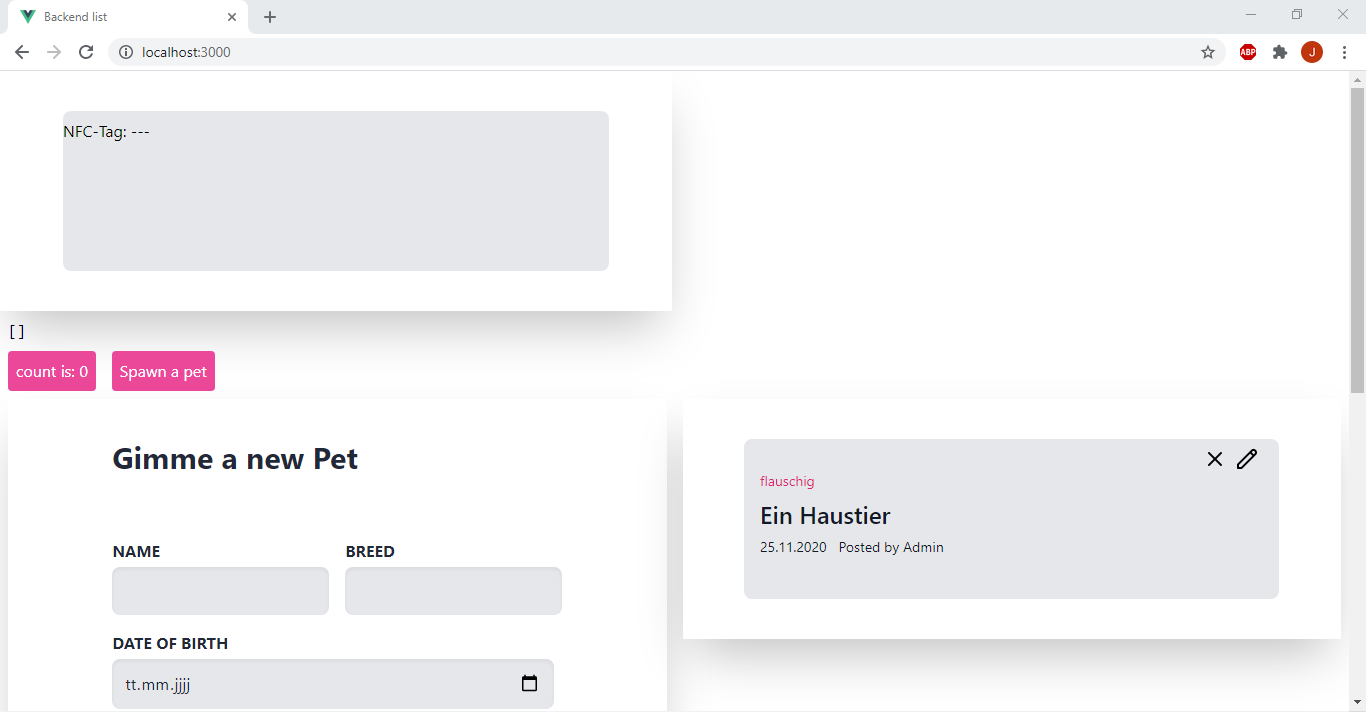
\includegraphics[width=\textwidth]{Haustiere.png}
    \caption{Zwei der Haustiere und die Anzeige des NFC-Readers}
    \label{Haustiere}
\end{figure}

\paragraph*{NFC-Tags auslesen} $~$ \\
Neben der Umsetzung des Hello-Worlds sollte sich mit dem Raspberry Pi und dem NFC-Reader auseinandergesetzt und das Auslesen der NFC-Tags implementiert werden. Diese Anforderung geriet mangels ausreichender Notizen beim ersten Review vorerst
in Vergessenheit, sodass sich das Team einige Tage vor Sprintende nicht sicher war, ob diese Anforderung bis zum Review umgesetzt werden könnte.
Um das Sprintziel nicht zu gefährden, mussten gegen Ende des Sprints Überstunden geleistet und das Feature konnte ins Produktinkrement aufgenommen konnte.
\\
Zur Umsetzung wurde im Backend die Klassen und der Service zur Verwaltung eines NFC-Readers und NFC-Tags
analog zu dem in \ref{HelloWorld} beschriebenen Vorgehen erstellt.
Außerdem wurde der Microservice \textit{nfc-reader} in der Projektstruktur unter \textit{packages}
angelegt. Dieser nutzt die Bibliothek \textit{Evdev}\footnote{https://github.com/PixnBits/node-evdev}, welches ein Interface für die Events der angeschlossenen
Eingabegeräte vom Linux-Kernel, wie in unserem Fall den NFC-Reader, bereitstellt. Dies ist möglich, da der NFC-Reader sich wie eine Tastatur verhält. Er
simuliert dabei eine Tastatureingabe mit dem Text der NFC-Tag-ID. Zur Nutzung wurden zwei Klassen erstellt. Zum einen die NFC-Reader Klasse
(im NFC-Reader Package), welche jeden simulierten Tastendruck des NFC-Readers abfängt, bis ein Zeilenumbruch (0A HEX) empfangen
wird und anschließend ein Event auslöst, welches die eingescannte ID beinhaltet. Die Hauptklasse nimmt dieses Event entgegen (Event-Listener) und setzt mittels des
NFC-Reader Services den aktuell anliegenden Tags (\textit{currentTag}) auf die übergebene ID. Durch die Nutzung von \textit{Web-Sockets} und \textit{Vue.js}
kann diese Änderung sofort im Frontend angezeigt werden. Aufgrund der potentiell hohen Komplexität des Abspielens von Musik wurde diese Funktionalität für den
folgenden Milestone eingeplant und vorerst lediglich die Anzeige der NFC-ID als JSON-String umgesetzt.
\\
Für den Microservice wurde anschließend ein Docker-Image kreiert, welches eine einfache und gleichzeitig optionale Auslieferung zur restlichen Installation
ermöglicht. Dies bringt den Vorteil, dass auch auf einem anderen System (wie z. B. einem esp32) integrierte NFC-Reader, statt des aktuellen genutzt werden können.

\paragraph*{Prototyping der Beutzeroberfläche} $~$ \\
Damit die Entwicklung zeitnah starten konnte, wurden die ersten Mockups für die Benutzeroberfläche erstellt.
Mithilfe des Prototyping-Tools \textit{figma} (vgl. \ref*{figma}) wurden Prototypen für die Start- , die Hauptansicht und die Ansichten
für das Bearbeiten und Anlegen von NFC-Tags erstellt (Eine Übersicht über das erstellte Design ist im Anhang unter \ref*{FigmaDesigns} zu finden).
Nach dem Design wurden die Ansichten in \textit{Click-Dummys} umgewandelt, um dem Kunden im folgenden Review einen Überblick über das Verhalten der
Benutzeroberfläche zu verschaffen.

\paragraph*{Review} $~$ \\
Dank des großen Engagements und der Bereitschaft Überstunden zu leisten, konnte dem Kunden zum Review ein neues Produktinkrement übergeben werden.
Das Produkt wurde um ein erstes User Interface erweitert, welches die Tag-ID vom angelegten NFC-Tags anzeigen konnte.
Der NFC-Reader wurde mit dem Raspberri Pi verbunden und als ein auslieferbares Docker Image bereitgestellt.
Auch wurden für die Entwicklung automatisierte Tests erstellt, welche neuen Code auf etablierte Code-Konventionen und Lauffähigkeit überprüften.

\paragraph*{Retrospektive} $~$ \\
Vor allem der Einsatz und das Know-How vom Teammitglied Anton wurde hier wertgeschätzt, welcher sich um die Automatisierung von Tests und Deployment kümmerte.
Auch das Gruppenklima wurde sehr gelobt und angemerkt, dass die Zusammenarbeit, Kommunikation und die regelmäßigen Meetings sehr positiv wahrgenommmen wurden.
Das Team konnte bei der Umsetzung dieses Meilensteins viel über die Funktionsweise der Frameworks \textit{Feathers}, \textit{Vue.js} und \textit{Tailwind} lernen.
Darüber hinaus kamen viele das erste mal Automatisierungsprozessen, Code-Reviews und Pull Request in Kontakt.
Das Team bemängelte bei dem Meilenstein aber auch, dass der Kundenwunsch zu spät behandelt wurde und die Prioritäten falsch gesetzt wurden.
Somit wurde als Verbesserungen für die nächsten Meilensteine eine bessere Koordination und Aufgabenverteilung vorgeschlagen.

\subsection{Meilenstein 3}
Vom 25.11.2020 bis zum 17.12.2020 fand die Umsetzung von Meilenstein drei statt.

\paragraph*{Mockup Überarbeitung} $~$ \\
Die erstellten Mockups für die Benutzeroberfläche sollten in diesem Sprint basierend auf dem Feedback von macio finalisiert werden.
Das Ergebnis führte bei den Entwicklern anfänglich zu etwas Unsicherheit, da das Team nur aus Studierenden des Studiengangs
Informationstechnologie bestand, welche mit dem Thema Usability, abgesehen von dem Modul
\textit{Usability Engineering}\footnote{\raggedright\url{https://moduldatenbank.fh-kiel.de/de-DE/Module/Details/0de99d45-efc9-437a-a190-24d539b2a1d8}},
wenig Kontakt haben und darüber hinaus wenig persönliche Erfahrungen in dem Themenbereich gesammelt hatten.
Diese Schwierigkeiten wurden durch offene Kommunikation an macio weitergegeben,
 die daraufhin einen ihrer Designer zur Unterstützung bei der Entwicklung bereitstellten.

\wrapfiguresafe{r}{0mm}{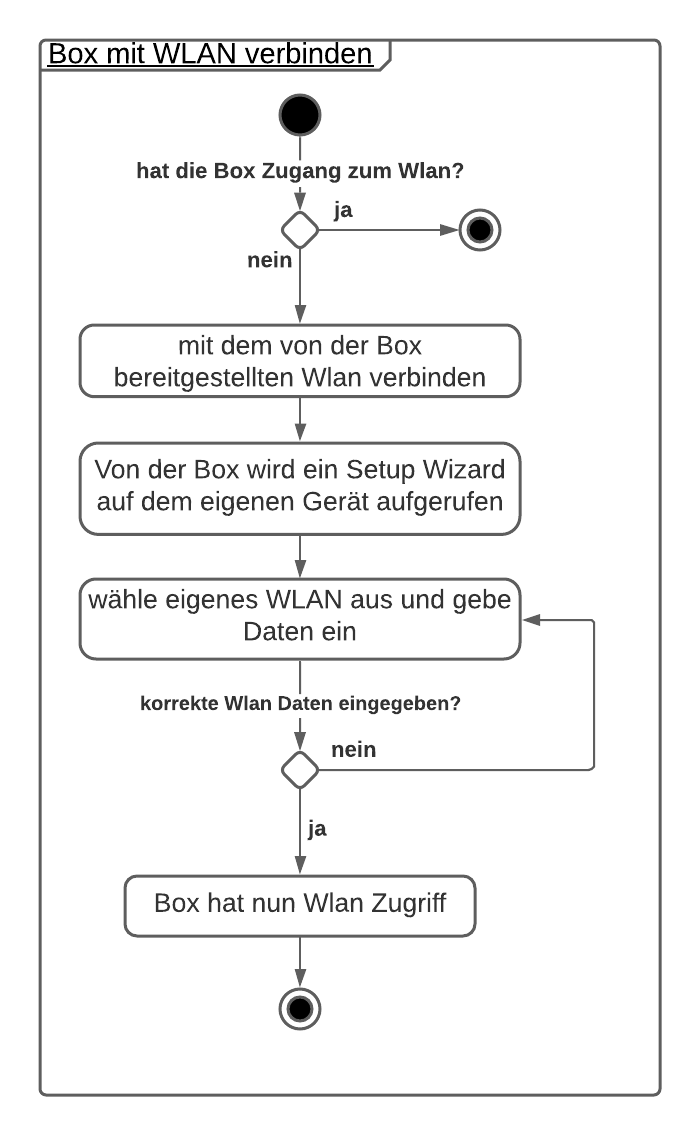
\includegraphics[width=0.45\textwidth]{ConnectToWIFI.png}}{Flowchart: Connect to WIFI}
\paragraph*{Flow-Charts} $~$ \\
Außerdem wurden die im letzten Sprint erstellten \textit{User Stories} als Grundlage für die Entwicklung von \textit{Flow-Charts} verwendet.
Diese wurden mit dem Online-Tool \textit{Lucidchart} (vgl. \ref*{Lucidchart}) erstellt und sind im Anhang unter \ref*{FlowCharts} zu finden.
Sie erleichterten die Umsetzung der Design-Mockups, indem sie notwendigen Abläufe visualisierten.
Dank dieses Zwischenschrittes konnten auch die nicht durch Mockups visualisierte Funktionen, wie das Verbinden der Box mit dem WLAN, zuerst logisch skizziert
werden, bevor sie programmiert wurden. Dadurch konnte innerhalb des Teams auführlich die beste Methode diskutiert werden, um die bestmögliche Usability
für den Benutzer sicherzustellen. Außerdem konnten sie auch dem Kunden vorgelegt werden, um etwailige Miskommunikation bei der Anforderungsanalyse zu vermeiden
und so die Wahrscheinlichkeit auf spätere Änderungen wichtiger Funktion zu senken. Die Erstellung dieser \textit{Flow-Charts} hat mit übereinstimmender
Meinung aller Teammitlgieder die spätere Programmierung maßgeblich effizienter gestaltet und wurde auch vom Kunden sehr geschätzt.


\paragraph*{Musik abspielen} $~$ \\
Auch der vom Kunden geäußerte Wunsch, beim Einlesen eines NFC-Tags die entsprechende hinterlegte Musik abzuspielen, sollte in diesem Milestone umgesetzt werden.
Dafür setzte sich ein Teil des Teams intensiv mit der \textit{Spotify-API}\footnote{https://developer.spotify.com/documentation/web-api/} auseinander.
Hierbei entdeckten die Entwickler die Bibliothek \textit{Spotify Web API node} (vgl. \ref*{SpotifyWebApiNode}), welche den Zugriff auf die \textit{Spotify-API},
abstrahiert und so den Zugriff auf diese erleichtert. Die Bibliothek wurde in Kombination mit \textit{Feathers-Hooks}
\footnote{https://docs.feathersjs.com/api/hooks.html} verwendet. Hooks sind Funktionen, die z. B. vor oder nach einem Feathers Service Aufruf ausgeführt werden
können. In diesem Fall beinhaltet der angelegte \textit{playSpotify} Hook einen Aufruf der Methode \textit{play} der \textit{Spotify Web API Node}, die den Song
hinter der \textit{URL} des mitgegebenen NFC-Tags abspielt. Dieser Hook ist an die \textit{patch} Methode es NFC-Reader Services angehängt, sodass dieser im
Anschluss an die \textit{patch} Methode, die den Eintrag des \textit{attachedTag} des NFC-Readers aktualisiert, aufgerufen wird.

\paragraph*{NFC-Tags scannen emulieren} $~$ \\
Da während des Projekts nicht alle Entwickler kontinuierlichen Zugang zu einem NFC-Reader hatten wurde im Zuge dieses Milestones außerdem die Möglichkeit
geschaffen, das Scannen eines NFC-Tags zu emulieren. Hierfür wurde ein \textit{Shell-Script} erstellt, welches einen \textit{HTTP PATCH request} an
das Backend schickt. Dadurch wird der \textit{attachedTag} des NFC-Readers auf Basis eines übergebenen Parameters gesetzt. So kann zum Beispiel ein NFC-Tag mit
der ID 12345 emuliert werden, indem im Terminal der Aufruf \textit{./simulate-read.sh 12345} durchgeführt wird, ohne dass der Entwickler einen physischen NFC-Reader
an seiner Entwicklungsmaschine angeschlossen haben muss. So konnten Funktionen wie das Anlegen eines neuen NFC-Tags von jedem Entwickler durchgeführt werden.


\paragraph*{Entwicklung des Welcome Screens mit Authentifizierung} $~$ \\
\wrapfiguresafe{r}{0mm}{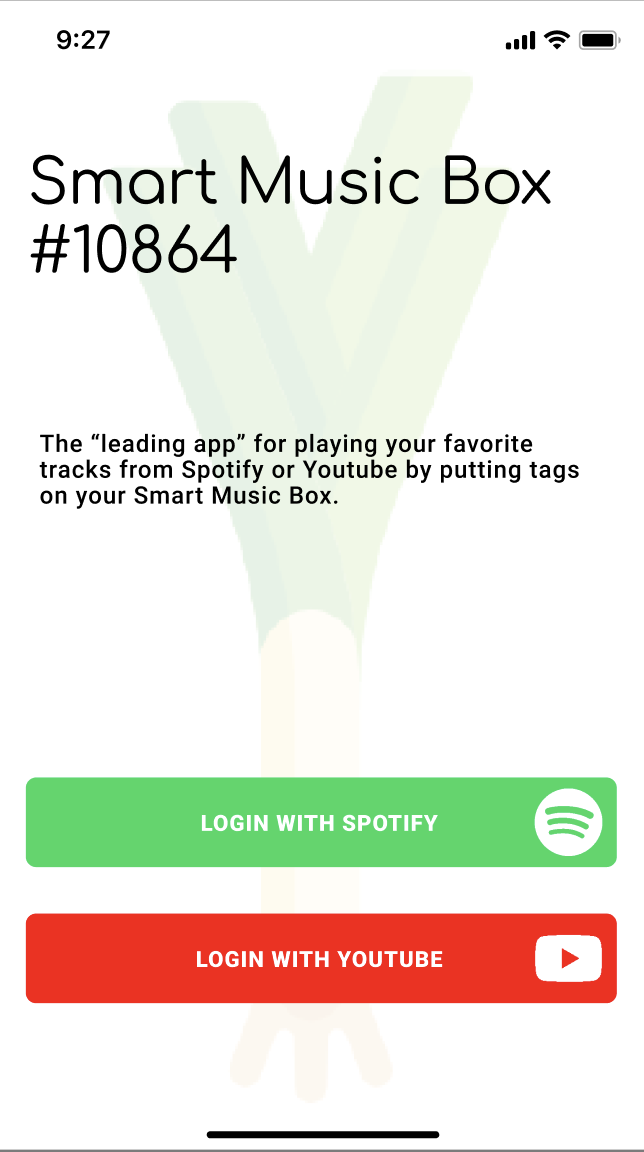
\includegraphics[width=0.45\textwidth]{WelcomeScreenV1.png}}{Welcome Screen Version 1}
Um das in diesem Milestone erstellte Feature des Abspielens von Musik sinnvoll nutzen zu können, musste sich auch mit der Authentifizierung mit Spotify beschäftigt
werden. Dafür wurde das offene Protokoll \textit{OAuth} verwendet, welches bereits in \textit{Feathers} abstrahiert implementiert ist. Zur Nutzung dieses
Protokolls wurde eine sogenannte \textit{Stragegy} angelegt, welche den für die Anmeldung notwenigen Datenaustausch mit Spotify ermöglicht.
Die dafür nötige \textit{Stragegy} mit dem Namen \textit{SpotifyStrategy} wird durch eine Klasse realisiert, welche von der Feathers bereitgestellten Klasse
\textit{OAuthStragegie} erbt. Bei der Anmeldung eines Benutzer wird von Spotify ein JWT-Token an das Backend übergeben. Ein JWT-Token besteht aus einem Base64
enkodiertem Text, welcher beliebige Daten beinhalten kann. Diese Daten sind unverschlüsselt (nur enkodiert) in dem Token hinterlegt und werden
durch eine Signatur auf ihre Integrität überprüft. Der von Spotify übermittelte JWT-Token enthält in diesem Fall die ID, E-Mail und den Namen des
Benutzers. Diese Daten werden extrahiert und sofern der Benutzer nicht bereits in der Datenbank vorhanden ist, zum Anlegen eines neuen Benutzers verwendet.
Sollte der Benutzer jedoch bereits in der Datenbank existieren, so wird dieser gegebenenfalls aktualisiert. Da sich jeder Benutzer vor der Verwendung der App
zuerst  mit einem gültigen Token identifizieren muss, wird bei möglichen Änderungen der Stammdaten in Spotify sofort immer der Datenbankeintrag in Feathers
aktuell gehalten.
\\~\\
Zum Beginn der Umsetzung wurde auf Basis des Mockups ein View in der Benutzeroberfläche (\textit{app} package) erstellt. Dieser enthält als Steuerelemente Infos
über den Namen des Produkts - \textit{leek-box} - und einen kurzen Untertitel, sowie einen \glqq Anmelden mit Spotify\grqq{} Button, der den OAuth-Prozess startet.
Diese Seite wurde mittels des \textit{Vue Routers} so konfiguriert, dass sie nur aufgerufen wird, wenn der Benutzer nicht angemeldet, also kein JWT-Token
vorhanden ist. Ist ein JWT-Token vorhanden, wird der Nutzer bei dem versuchten Aufruf dieser Seite automatisch auf die Hauptseite weitergeleitet.

\paragraph*{Veröffentlichung der App auf Github Pages} $~$ \\
Zur Veröffentlichung unseres Frontends der \textit{leek-box} verwenden wir den Dienst Github Pages welcher ein Webhosting von statischen Dateien unter einer xyz.github.io URL anbietet.
Das Team verwendete für das Frontend ein separates Repository \textit{project-leek/project-leek.github.io} mit der URL project-leek.github.io.
Nach dem Continous-Delivery Verfahren, baut die Pipeline des eigentlichen project-leek Repositories automatisch nach jedem Merge auf den master Branch das \textit{app-package}.
Dafür wird das Build-Tool des \textit{app-package}s aufgerufen und die dabei enstanden statischen Dateien werden von dem Pipeline Plugin
\textit{github-pages-deploy-action}\footnote{\raggedright\url{https://github.com/JamesIves/github-pages-deploy-action}} aus der Pipeline in das separate
\textit{project-leek/project-leek.github.io} Repository für den GitHub Pages Dienst kopiert. Somit befindet sich unter project-leek.github.io immer die aktuellste Version der App.
Dies hat den Vorteil, dass Änderungen wie zum Beispiel Bugfixes und neue Features dem Endanwender schnellst möglich zur Verfügung gestellt werden können ohne das auf einen Release-Plan Rücksicht genommen werden muss.

\paragraph*{Review \& Retrospektive} $~$ \\
Zusätzlich zu dem Wunsch, beim Anlegen eines NFC-Tags die jeweilig hinterlegte Musik abzuspielen, war zum Review auch das Einloggen
in einen bestehenden Spotify Account möglich. Jegliche Neuerung auf dem Master wurden außerdem auch auf Github.io veröffentlicht, sodass der Kunde jederzeit
den Fortschritt ermitteln konnte.
\\
Die vom Team durchgeführte Retrospektive ergab, dass die Problembewältigung durch die Anwendung von Pair Programming in diesem Sprint optimiert werden konnte.
Auch der Workflow mit Github und den Pull Request wurde verinnerlicht sowie Code Reviews verstärkt durchgeführt. Das Team lernte in diesem Sprint
Vue Hooks und die Stärken von Feathers in Verbindung mit OAuth kennen. Festgestellt wurde außerdem, dass einige Tickets weiterhin stark voneinander abhängig waren,
weshalb das Bearbeiten einiger Aufgaben nicht direkt möglich war. Da Abhängigkeiten teilweise unvermeidbar sind, wurde sich geeinigt, diese Tickets bei hoher
Komplexität mittels Pair-Programming umzusetzten, um sie möglichst schnell und qualitativ umsetzten zu können. Um das Risiko der Entstehung zukünftiger Probleme
zu senken wurde außerdem festgelegt mögliche Problemstellungen nicht erst im Standup, sondern so früh wie möglich mitzuteilen. Genauso sollte neu gelerntes besser
kommuniziert werden, um die Arbeit effizienter zu gestalten. Hierfür wurden die \textit{Standups} als Rahmen gewählt.

\subsection{Meilenstein 4}
%Ziel
Zu beginn dieses Meilensteins waren alle Grundlagen gelegt um mit der Umsetzung der Hauptfunktionen zu beginnen.
Es sollten möglichst viele Teile des designten User Interfaces umgesetzt werden, allerdings lag der Fokus auf einem vollständigem \glqq Add-Tag-Flow\grqq.
Dazu gehörten:
\begin{enumerate}
  \item Scannen des Tags
  \item Vergeben eines eigenen Namens
  \item Auswählen von Musik
  \item Auswählen eines eigenen Bilds
\end{enumerate}
Weiterhin sollten für den nächsten Schritt die Mockups erstellt werden, wie ein Nutzer den Lautsprecher zur Wiedergabe auswählt sowie seine eigene \textit{Leek Box} initial einrichtet.

Um paralleles Arbeiten und Eigenständigkeit der Tickets zu ermöglichen, wurde jede Ansicht in ihre einzelnen Komponenten aufgeteilt.
Diese Komponenten sollten für sich alleine stehend funktionieren und so anpassbar sein, dass z.B nur ein Button Komponent entwickelt werden musste, dass auf
allen Ansichten verwendet werden konnte. Es wurde daher erst die grundliegenden Komponenten wie Buttons, Textfields und Dropdowns entwickelt um aus diesen
Komponenten Views zu erstellen.

Die Views wurden ebenfalls so in Tickets aufgeteilt, dass möglichst parallel gearbeitet werden konnte.
Beispielsweise wurde die Darstellung auf dem Homescreen und die Auswahl von Infos, Musik und Bild komplett unabhängig voneinander bearbeitet und mit Platzhalterdaten befüllt.
Schließlich wurden alle Komponenten und Seiten zusammengefügt um einen vollständigen Flow zu ermöglichen.
Es konnte nun erfolgreich per UI ein neuer Tag der Datenbank hinzugefügt und in dem HomeScreen angezeigt werden.

\wrapfiguresafe{r}{0mm}{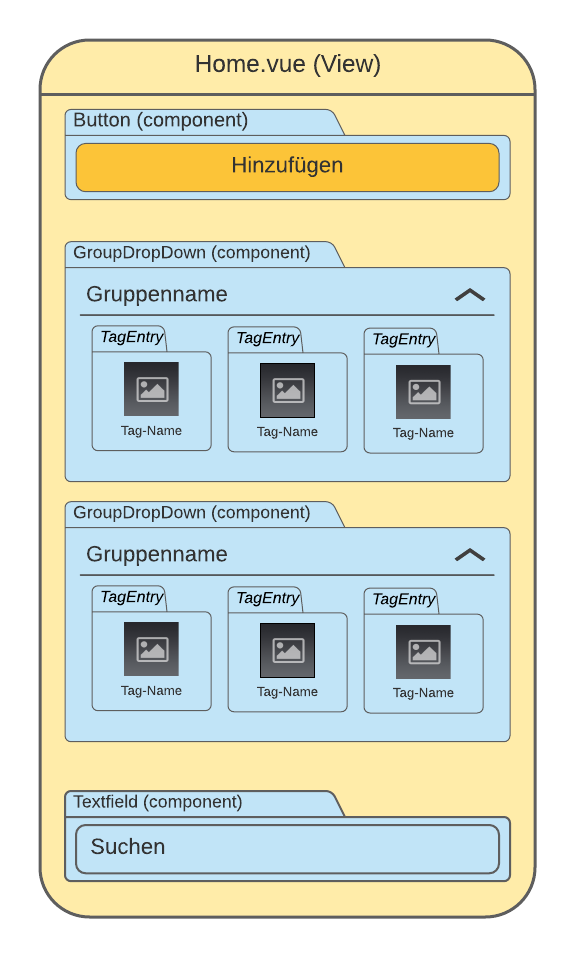
\includegraphics[width=5.9cm]{HomeScreenSchema.png}}{Schematischer Aufbau Home.vue aus \textit{components}}
\paragraph*{Components}$~$ \\
Für Elemente, die häufig in der Anwendung genutzt werden (Button, Textfield, DropDownList),
entwicklete das Team \textit{Vue Components}, die in dem Ordner \textit{uiBlocks} für alle Entwickler leicht zugänglich abgelegt wurden.
Diese \textit{components} garantieren, dass die Elemente anpassbar sind und dennoch einem einheitlichen Design folgen.
Besonders am Anfang halfen sie dem Entwickler, da sie die Komplexität der Implementierung von Design und Funktionalität senkten.
Diese mussten lediglich einmalig in der \textit{component} definiert werden und konnten dann bei Bedarf in den \textit{Views} eingebunden werden.
Es musste dann nur noch der Inhalt über \textit{properties} übergeben werden.
Während der fortschreitenden Entwicklung trat allerdings das Problem auf, dass immer mehr Anforderungen an die \textit{components} gestellt wurden,
 und damit immer mehr \textit{Properties} für deren Anpassung notwendig waren.
 Dies resultierte darin, dass zum Beispiel die \textit{Button-Component} sehr unübersichtlich wurde und redundanten Code enthielt.
Aufgrund der verschiedenen geforderten Größen und Anforderungen der enthaltenden Texte und Bilder,
 stieg die Anzahl der zu übergebenen Parameter immens, was zu deutlich niedriger Übersichtlichkeit führte.
Als Lösung wurde in späteren Meilensteinen eine erneute Analyse durchgeführt, um zu ermitteln, welche Anforderungen einzelne Komponenten erfüllen mussten.
Die Ergebnisse dieser Analyse wurden anschließend genutzt, um den Code zu überarbeiten, wodurch die Übersichtlichkeit der \textit{components} wiederhergestellt wurde.

\wrapfiguresafe{r}{0mm}{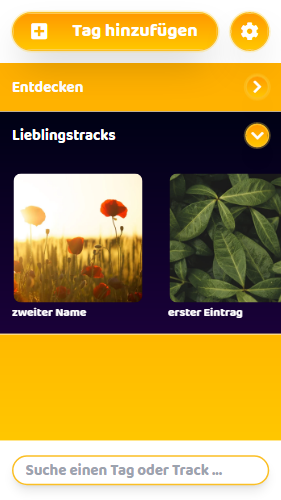
\includegraphics[width=4cm]{Home.png}}{Home View}
\paragraph*{Umsetzung des Homescreens}$~$ \\
Im HomeScreen sollten alle angelegten Tags gruppiert angezeigt werden. Hierfür wurden zwei \textit{components} angelegt. Die Erste (\textit{TagEntry})
enthält das Bild und den Namen eines NFC-Tags und kann in der Anwendung vielseitig wiederverwendet werden. Die Zweite \textit{component} mit dem Namen
\textit{GroupDropDown} repräsentiert eine Gruppe, zu der ein NFC-Tag gehört.
Pro NFC-Tag in der jeweiligen Gruppe wird eine Instanz der \textit{TagEntry component} in die Gruppe geladen.
Zusätzlich erhielt die \textit{GroupDropDown component} die Funktionalität auf- und
zuklappbar zu sein. \\
Diese \textit{components} werden in \textit{Home} angezeigt. Neben der Einbindung von einer \textit{GroupDropDown component} pro Gruppe
wurde im Kopfbereich noch die vom Team erstelle \textit{Button component} verwendet, die das Anlegen eines neuen NFC-Tags einleiten sollte.
Im Fußbereich befindet sich eine Suchleiste, die das Filtern der angezeigten NFC-Tags ermöglichen soll.
Die beiden letztgenannten Features waren zu diesem Zeitpunkt noch nicht umgesetzt.

\paragraph*{Entwicklung der \glqq Tag hinzufügen\grqq{} Funktionalität}$~$ \\
Um dem Benutzer das Hinzufügen von neuen NFC-Tags zur ermöglichen, wurde eine neue \textit{View} mit dem Namen \textit{AddTag} erstellt, welche wie auch
die \textit{Home}-View in Kopf-, Haupt- und Fußbereich eingeteilt ist. Beim Laden der View wird eine neue Instanz der Klasse \textit{NFC-Tag} erstellt.
\\~\\

\begin{minipage}{\textwidth}
  \begin{lstlisting}[caption={Dynamisches Laden der components von AddTag}, captionpos=b]
    <component
      :is="steps[activeStep].component"
      v-model:nfc-tag="nfcTag"
      @update:is-valid="dataValid = $event"
      @proceed="nextStep"
    />
  \end{lstlisting}
\end{minipage}

Im Hauptbereich der \textit{View} werden die vier \textit{components}, die für die Eingabe der NFC-Tag Daten zuständig sind, dynamisch geladen.
Hierfür wird der beim Laden erstellte NFC-Tag (\textit{newTag}) an alle \textit{components} nacheinander weitergegeben und in ihnen mit Informationen gefüllt.
Der Fußbereich enthält abhängig von der im Hauptbereich gerade aktiven \textit{component}, \textit{Button components} für \glqq Zurück\grqq{}, \glqq Weiter\grqq{} und
\glqq Anlegen\grqq.
Alle der folgenden \textit{components} beinhalten Validierung für die eingegebenen Daten, sodass sichergestellt wird, dass das \textit{newTag} jederzeit gültige Daten besitzt.
Bei Änderung der Werte in den \textit{components} wird das Event \textit{update:is-valid} ausgelöst und in \textit{AddTag} die\textit{Disabled}-Eigenschaft des sich in der Fußzeile befindliche Button abhängig vom der Gültigkeit verändert.
So kann in jedem Schritt nur fortgefahren werden, wenn alle Eingaben die korrekte Form haben.
Alle diese \textit{components} werden ebenfalls für die Bearbeitung der NFC-Tags wiederverwendet.
\\~\\
%AddStepScan
\wrapfiguresafe{r}{0mm}{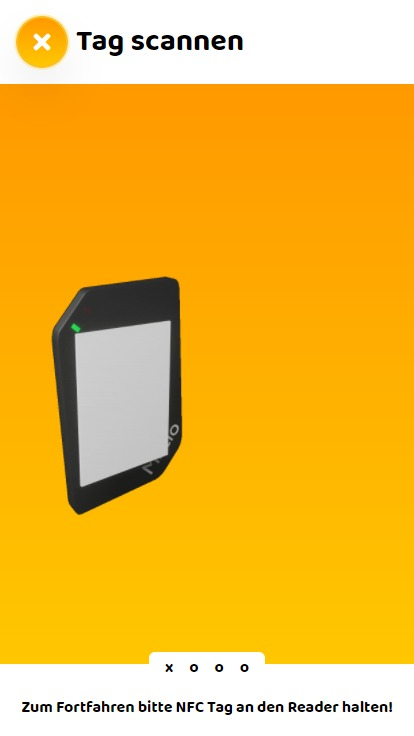
\includegraphics[width=4cm]{AddStepScan.jpeg}}{Step Scan (Add)}
Die Erste \textit{component}, welche in den Hauptbereich geladen wird, ist \textit{TagStepPlaceTagOnReader}. Dieser beinhaltet einen Text und ein \textit{GIF},
welches den Benutzer zum Scannen des NFC-Tags auffordert. Im \textit{TypeScript}-Code wird im \textit{Lifecycle Hook onMounted} an das \textit{patch}-Event des
NFC-Readers der Aufruf der Funktion \textit{attachedTagListener} gebunden. Wird nun ein NFC-Tag gescannt, führt der \textit{NFC-Reader Microservice} mittels Feathers ein Update (Aufruf des \textit{Patch}-Events) auf den \textit{NFC-Reader} durch und setzt das Attribut \textit{attachedTag} auf die gescannte NFC-ID.
Anschließend wird geprüft, ob ein NFC-Tag mit dieser ID bereits in der Datenbank vorhanden ist und der Benutzer in diesem Fall an die \textit{View} zum Bearbeiten des Tags weitergeleitet.
Ist der NFC-Tag noch nicht angelegt, wird die ID an die \textit{ID-Property} des \textit{newTag} gebunden und die Events \textit{update:nfc-tag} und \textit{proceed} ausgelöst.
\textit{update:nfc-tag} bewirkt, dass das Attribut \textit{TagId} des \textit{newTag} gesetzt wird.
\textit{proceed} weist \textit{AddTag} an, die nächste \textit{component} in den Hauptbereich der \textit{View zu laden}.
Dabei wird die Funktion \textit{attachedTagListener} vom \textit{patch}-Event abgemeldet.
\\~\\
%AddStepInfo
\wrapfiguresafe{r}{0mm}{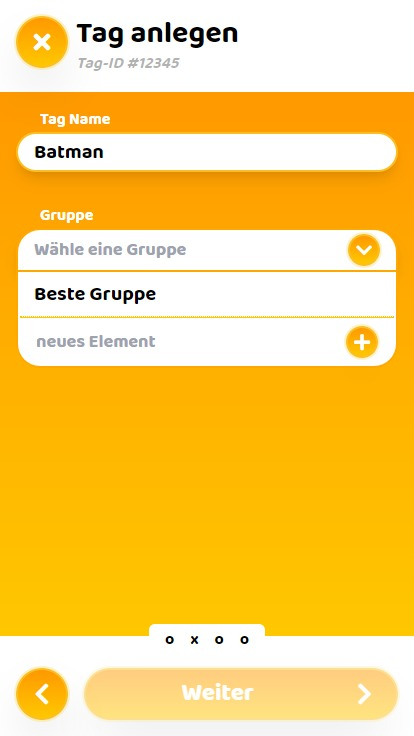
\includegraphics[width=4cm]{AddStepInfo.jpeg}}{Add Step Scan-Tag}
Als Nächstes wird die \textit{TagStepInfo component} geladen.
Sie beinhaltet eine \textit{Textbox component} für den Namen des NFC-Readers.
Diese erhält als \textit{v-model} eine \textit{computed property}\footnote{\url{https://v3.vuejs.org/guide/reactivity-computed-watchers.html}}.
Diese ruft im \textit{setter} die Methode \textit{updateTag} auf, welche die zwei Parameter \textit{key} und \textit{value} erwartet, um die Eigenschaft \textit{key} (in diesem Fall \glqq name\grqq{}) auf den im Parameter \textit{value} übergebenen Wert zu setzten.
Als Zweite \textit{component} kommt ein \textit{DropDown} zum Einsatz,
welches die Auswahl der Gruppe ermöglicht. Hierbei kann sowohl aus bereits bestehenden Gruppen gewählt, als auch direkt in der \textit{component} eine neue erstellt
werden. Auch hier wird die Methode \textit{updateTag} verwendet, die in diesem Fall mit dem Wert \glqq group \grqq{} für den Parameter \textit{key} aufgerufen wird. Der eingegebene Name und die Gruppe werden an die jeweiligen Eigenschaften von \textit{newTag} gebunden und das Event \textit{update:nfc-tag} aufgerufen, wodurch die \textit{View AddTag} den Wechsel zur nächsten \textit{compontent} einleitet.
\\~\\
%AddStepTrack
\wrapfiguresafe{r}{0mm}{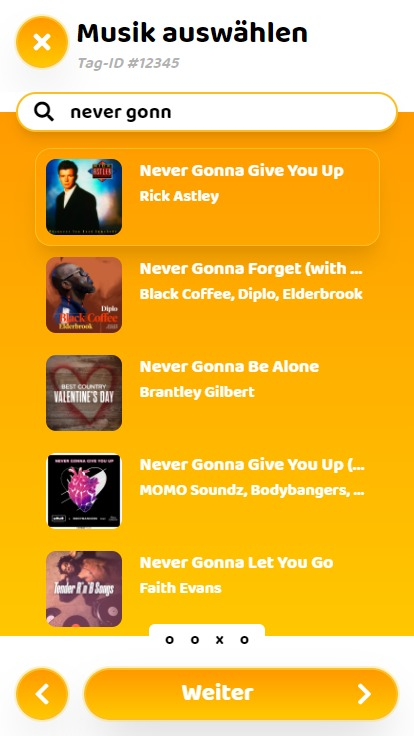
\includegraphics[width=4cm]{AddStepTrack.jpeg}}{Add Step Track}
Hier in der \textit{TagStepTrack} erhält der Benutzer die Möglichkeit, den Song auszuwählen, der beim Scannen des NFC-Tags abgespielt werden soll.
Der gewünschte Song-Titel oder Suchwörter können in eine \textit{Textbox component} eingeben werden. Zum Abrufen der Songs von Spotify wurde der \textit{SpotifyTrackService} erstellt, in dem die Methode \textit{find} überschrieben wurde.
Diese beinhaltet den Aufruf der Funktion \textit{searchTracks} der \textit{Spotify Web Api}, welcher als Parameter der in der Suchtextbox eingegebene Text übergeben wird.
Für jeden zu dem übergeben Text passenden Titel wird dann eine Instanz der erstellten Klasse \textit{Track} erstellt, die Informationen über die \textit{URL}, den Titel, die \textit{Bild-URL}, und die Künstler erhält. Das Array mit den passenden \textit{Track}-Instanzen wird anschließend an \textit{TagStepTrack} zurückgegeben und die Infos mit Bild, Titel und Interpreten angezeigt. Die Auswahl erfolgt dann per Klick auf den gewünschten Song.
Bestätigt wird die Auswahl per Klick auf \glqq Weiter\grqq{} in der Fußzeile.
Dadurch wird \textit{update:nfc-tag} Event ausgelöst und die letzte \textit{component} in die \textit{AddTagView} geladen.
\\~\\
%AddStepImage
\wrapfiguresafe{r}{0mm}{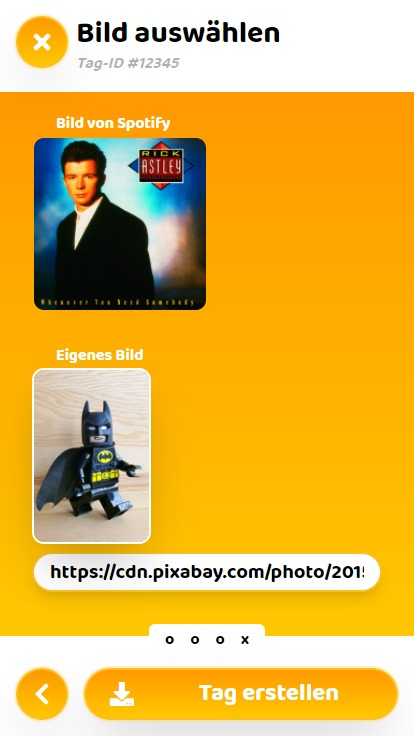
\includegraphics[width=4cm]{AddStepImage.jpeg}}{Add Step Image}
Zuletzt kann im \textit{TagStepImage} das gewünschte Bild für den NFC-Tag ausgewählt werden.
Standardmäßig wird hier das Albumcover des Songs ausgewählt, welches in \textit{AddStapTrack} bereits gesetzt wurde.
Um sicherzustellen, dass die Albumcover jederzeit aktuell sind, wird in der Datenbank nicht das Bild, sondern lediglich die URL des Bildes gespeichert.
Sollte der Musik-Streaming-Anbieter dieses ändern, wird so automatisch auch das Albumcover in der Applikation geändert.
Dies hat außerdem den Vorteil, dass die Anwendung wesentlich speicherplatzeffizienter ist, da statt teilweise sehr großen Bilddateien jeweils nur die URL gespeichert wird.
Um dem Benutzer mehr Freiheiten in der Gestaltung zu geben, kann alternativ auch ein eigenes Bild verwendet werden.
Dieses muss in der aktuellen Version auf einem Online-Dienst vorliegen.
Ist dies gewünscht, kann in einer entsprechenden Textbox die \textit{URL} dieses Bildes eingetragen werden, worauf das Bild automatisch zur Vorschau in ein dafür vorgesehenes Vorschaufeld geladen wird.
Dies stellt sicher, dass der Benutzer nicht versehentlich eine falsche Bild-URL wählt.
Zusätzlich wird diese Textbox zusätzlich mittels eines \textit{RegEx} geprüft, um sicherzustellen, dass es sich um eine nutzbare Bilddatei handelt.
Zur Bestätigung muss entweder auf das Albumcover oder auf das eigene Bild geklickt werden.
Das Erstellen des Tags kann dann mit einem Klick auf \glqq Anlegen\grqq{} im Fußbereich der \textit{View} abgeschlossen werden.
%Probleme
Durch die angestrebte Unabhängigkeit musste besonders viel Arbeit investiert werden, um die Features miteinander zu verbinden.
Dieser Prozess dauerte länger als erwartet und forderte eine hohes Maß an Kommunikation zwischen den Teammitgliedern.
Teilweise enstanden Wartezeiten und funktionierender Code wurde, über mehrere Merges, unstabil oder defekt.
Kurz vor dem Review musste noch viel getan werden, um eine reibungslose Präsentation zu garantieren.

%Lösungen
Nachdem die ersten großen Merges abgeschlossen wurde, entschied das Team eine interne und anonyme Evaluation der Teammitglieder zu starten.
Jedes Teammitglied hatte somit konstruktive Kritik aber auch Lob und Unterstützung erhalten und konnte an den eigenen Schwächen arbeiten und Stärken weiter ausbauen.
Darüber hinaus wurde auch beschlossen, in den folgenden Sprints die Menge an zu bearbeitenden Issues besser festzulegen.
%Product Increment
Das Produkt wurde um die Grundfunktionen erweitert.
Es ist nun möglich, Tags anzulegen und entsprechend den Namen, Musik und ein Bild festzulegen.
Genauso ist es dem Nutzer nun möglich, alle angelegten Tags zu durchsuchen.
Es wurde weiterhin auch das Design Mockup von dem von macio gestellten Designer in Vue größtenteils umgesetzt.
Für die Entwickler wurden auch die automatisierten Tests um einen Test auf Typsicherheit erweitert.
%Retrospektive
Besonders gut gefiel dem Team das Teamklima, vor allem des ehrliche Miteinander.
Trotz Komplikationen und Probleme konnte dem Kunden am Ende ein funktionierendes Product Increment geliefert werden.
Pull Requests und Tickets wurden besser beschrieben, sodass Probleme verständlicher waren.
Vor allem durch das interne Team Review wurde die Zusammenarbeit weiter verbessert.
Das Team konnte das Wissen zu Vue, vor allem die Themen Reaktivität, Events und Kommunikation zwischen Komponenten ausbauen.
Insgesamt war das Zeitmanagement verbesserungswürdig, da sich für einzelne Tickets zu viel Zeit genommen wurde.
Das Team stimmte überein, dass eine bessere Planung sowie Abstimmung für die nächsten Meilensteine notwendig wäre.
Auch sollte eine frühere interne Deadline gesetzt werden, damit nicht kurz vor dem Sprintende noch viele Fehler auftreten und behoben werden müssen.
Um insgesamt auch die Arbeit kontinuierlicher zu gestalten, sollten Aufgaben in kleinere Probleme aufgeteilt werden.


\wrapfiguresafe{r}{0mm}{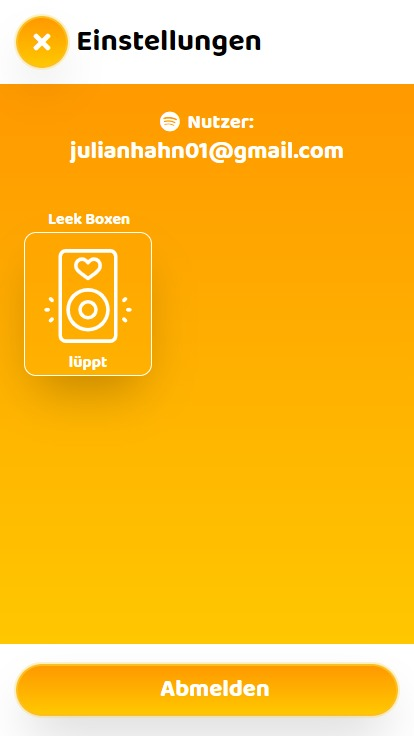
\includegraphics[width=0.45\textwidth]{Settings.jpeg}}{Leek Box Einstellungen}
\subsection{Meilenstein 5}
Mit dem fünften Meilenstein, der zwischen dem 14.01.2021 und 28.01.2021 stattfand, sollte die Entwicklung am Produkt weitgehend abgeschlossen werden, sodass der Fokus auf den Bericht gelegt werden konnte.

%Ziel
Geplant war die letzten Anwendungszenarien final umzusetzen, sodass die folgenden beiden Meilensteine zum Beheben kleinerer Fehler genutzt werden konnten.
Somit war das Ziel die Umsetzung einer \textit{View} für die Einstellungen der \textit{Leek Box}, als auch der Tags.
Außerdem sollten die User Interface Elemente, sofern noch nicht geschehen, ein einheitliches Design erhalten.
Die Dokumentation zur Bedienung der \textit{Leek Box} sollte fertiggestellt und mit der Arbeit am Bericht begonnen werden.
\\~\\
% Settings
Die \textit{View} für die Einstellungen der \textit{Leek Box} wurde hinzugefügt, die durch ein Zahnrad auf der Startseite aufgerufen werden kann.
In diesen Einstellungen können die Nutzer nun den Lautsprecher für die Wiedergabe auswählen und sehen, mit welcher Email-Adresse sie angemeldet sind. Außerdem enthält die Ansicht einen Button um sich auszuloggen.
\\~\\
% TagDetails
\wrapfiguresafe{r}{0mm}{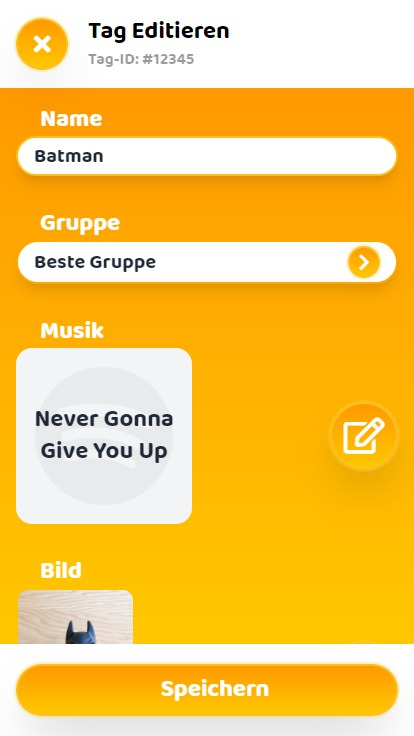
\includegraphics[width=0.45\textwidth]{TagDetails.jpeg}}{Tag Details}
Auch die Funktionalität zum Bearbeiten der NFC-Tags wurde in diesem Meilenstein umgesetzt.
An dieser Stelle zeigten sich erneut die Vorzüge von Frameworks wie \textit{Vue}, da somit die bereits vorhandenen \textit{components} wiederverwendet werden konnten.
Um ein gleiches Design der Überschriften der einzelnen Inputs zu garantieren, wurden die erstellten \textit{components} \textit{LabeledInput} für die Anzeige von Namen, Gruppe, Musik und Bild verwendet.
Zur Änderung des Namens wird das erstellte \textit{component} \textit{TextInput} genutzt, dem beim Aufruf der \textit{View} eine Referenz auf \textit{nfcTag.name} übergeben wird, sodass dieses den Namen anzeigt.
Ähnlich erfolgt die Auswahl und Anzeige der Gruppe. Hier wird anstatt der \textit{TextInput component} die \textit{Dropdown component} verwendet, die eine Referenz auf \textit{nfcTag.Group} empfängt und als Elemente die bereits existierenden Gruppen enthält.
Der Benutzer hat ebenfalls die Möglichkeit neue Gruppen anzulegen.
Für die Anzeige des dem Tag zugewiesenen Musikstücks wird ein dem \textit{TagEntry compontent} visuell ähnliches Element verwendet, welches als Hintergrund das angedeutete Logo des Musikstreaming-Anbieters enthält.
Zur Änderung des Musikstücks ist die Bearbeiten-Schaltfläche (\textit{Button component}) vorgesehen, die den Benutzer auf die bereits beim Anlegen verwendete \textit{component AddStepTrack} weiterleitet, die die benötite Funktionalität liefert.
Das gleiche Verfahren wird auch für die Anzeige und Änderung des Bildes verwendet.


% Visualisierung des ausgewählten Tags
Um dem Nutzer zu signalisieren, ob ein Tag ausgewählt wurde, wurde in \textit{Home.vue} ein weiteres Attribut \textit{selectedTag} angelegt.
Jedem Tag-Element auf der Startseite wurde ein \textit{OnClick Listener}, welcher bei einem Klick das jeweilige Element als \textit{selectedTag} setzt hinzugefügt.
\\~\\
\begin{minipage}{\textwidth}
  \begin{lstlisting}[caption={Hervorgeben aus ausgewähltem NFC-Tag}, captionpos=b]
    const toggleTag = (tag: NFCTag): void => {
      selectedTag.value =
        tag === selectedTag.value ? null : tag;
      buttonTransitionActive.value = true;
    };
  \end{lstlisting}
\end{minipage}
Um dynamisch die CSS-Klasse der ausgewählten Tags zu ändern, wurde an dieser Stelle bei den \textit{TagEntrys} der ternärer Operator genutzt.
Je nachdem ob der \textit{TagEntry} der gleiche wie der \textit{selectedTag} war, wurden diesem andere Klasseneigenschaften gegeben.
\\~\\
\begin{minipage}{\textwidth}
  \begin{lstlisting}[caption={Caption}, captionpos=b]
    <TagEntry
      v-for="entry in group.tags"
      :key="entry.nfcData"
      class="m-4 w-2/6 flex-shrink-0 text-4xl"
      :class="{ 'opacity-25': selectedTag !== entry &&
                              selectedTag !== null
              }"
      :img="entry.imageUrl"
      :name="entry.name"
      @click="toggleTag(entry)"
    />
  \end{lstlisting}
\end{minipage}
Wurde nun also ein Tag ausgewählt, wurden allen anderen die Klasse \lstinline{opacity-25} zugewiesen, was einer Tranzparenz von 25\% entsprach.

% Initial Setup
Im Sprint wurde auch das Produkt auf Auslieferbarkeit getestet, indem das komplette Setup durchgeführt wurde.
Dabei wurde ein Setup-Guide\footnote{https://github.com/project-leek/project-leek/blob/docs/Build.md} entwickelt, sodass andere Nutzer ihre eigene \textit{leek-box} bei sich einrichten könnten.

%Probleme
Wie bereits beim vorherigen Meilenstein gestaltete sich auch hier das Zeitmanagement schwierig.
Das Team hätte in diesem Sprint mehr Tickets umsetzen und dem Kunden präsentieren können, als zu Beginn versprochen. Jedoch fehlte die Zeit um die Features genügend zu testen und entsprechend fehlerfrei dem Kunden präsentieren zu können.
Somit beschloss das Team dem Kunden im Review nur die anfänglich geplanten Featuers vorzustellen und die zusätzlichen Tickets im nächsten Sprint zu vollenden.
Das Produkt konnte um die Einstellungen der \textit{Leek Box} und die \textit{TagDetails}  erweitert werden.
Auch der Setup Guide wurde fertiggestellt, sodass ein Nutzer selbstständig eine eigene \textit{Leek Box} einrichten könnte.
Bei dem Design wurden, bis auf ein paar Kleinigkeiten die im folgenden Milstone behoben wurden, alle Unstimmigkeiten beseitigt.

%Retrospektive
Das Team erhielt vom Kunden für das bisher entstandene Produkt viel Lob.
Da das Team viel Gefallen an dem Projekt gefunden und entsprechend viel Energie aufgewendet hat, war dieses Lob sehr wertvoll und motivierend.
Das Team konnte außerdem weitere Vue Funktionen kennenlernen.
Problematisch war es, dass manche Tickets von mehreren Entwicklern zeitgleich oder nacheinander bearbeitet wurden, sodass einige der getätigten Änderungen redundant waren.
Außerdem erfolgte die Kommunikation von größeren Änderung an jedes Teammitglied teilweise nur lückenhaft.
Nach der Retrospektive wurde dies dem Team deutlich und es wurde sich auf eine bessere Kommunikation geeinigt.
Lösungsvorschläge waren Verbesserung des Zeitmanagements durch Steigerung der Arbeitsstunden zu Beginn eines Sprints, sodass gegen Sprintende weniger offene Tickets vorhanden waren und das Team mehr Zeit zur Behebung möglicher Fehler vorhanden wäre.
Eine bessere Kommunikation konnte durch das Festhalten von größeren Änderungen in den Pull Requests und Markierung aller Gruppenmitglieder erreicht werden.

\subsection{Meilenstein 6}
Der sechste Meilenstein fand vom 28.01.2021 bis zum 15.02.2021 statt.
Mit diesem Sprint sollte das User Interface finalisiert, alle Fehlerbehebung abgeschlossen und somit die Entwicklung beendet werden, sodass der Fokus komplett auf den Bericht gelegt werden konnte.
So konnte der folgende und letzte Meilenstein für letzte Korrekturen am Bericht und das Vorbereiten der Projektpräsentation genutzt werden.
\\~\\
\wrapfiguresafe{r}{0mm}{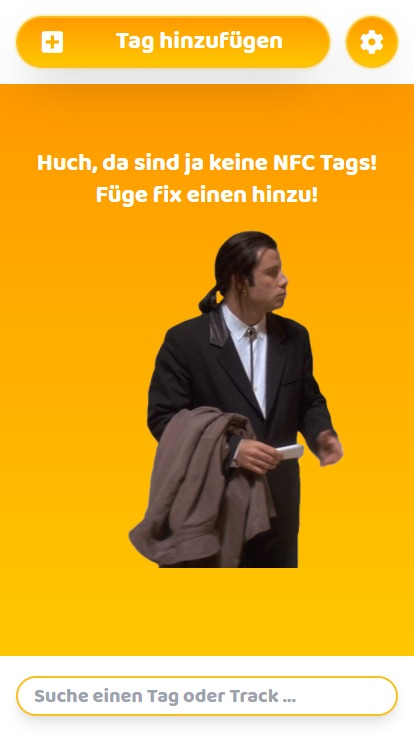
\includegraphics[width=0.45\textwidth]{HomescreenNoTags.jpeg}}{Startseite ohne Tags}
\paragraph*{Entwicklung} $~$ \\
Zu Beginn wurden die letzten Softwaretickets abgeschlossen. Vor allem am User Interface wurden noch letzte Änderungen durchgeführt.
Auf allen Seiten wurde die Höhe des \textit{Header} und \textit{Footer} auf die gleiche Größe angepasst. \\
Aus der Datenbank wurden die manuell generierten Einträge und die Methoden zum automatischen \textit{Seeding} der NFC-Tags gelöscht.
Auf der Startseite wurde dem User nun ein Hinweis angezeigt, falls dieser noch keine NFC-Tags angelegt hat. Hierfür wird beim Laden der NFC-Tags die Anzahl geprüft und im Falle von keinem vorhandenen Tags ein \textit{div} mit einem \textit{GIF} und eines Hinweistextes über konditionales Rendering per \textit{v-if} angezeigt oder ausgeblendet.

\paragraph*{Button Refactor} $~$ \\
Wie im Meilenstein vier bereits festgestellt, musste der häufig verwendete Button sehr anpassbar sein und in folgenden Versionen exisitieren:
\begin{itemize}
  \item nur Text
  \item Text mit Icon links vom Text
  \item Text mit Icon rechts vom Text
  \item ein Icon ohne Text
\end{itemize}
Um diese und andere Anforderungen zu erfüllen, stieg die Komplexität des Buttons, bedingt durch eine Vielzahl von übergebenen Parametern, stark.
Weiterhin musste die Größe des Buttons anpassbar, aber trotzdem möglichst einheitlich über die einzelnen Views hinweg, sein. Die \textit{component} wurde vom Team gründlich überarbeitet um redunanten Code zu vermeiden. Statt den bisher zwölf Parametern, konnten alle Anforderung auch mit acht Parametern erreicht werden.
\\
An dieser Stelle soll verdeutlicht werden, wie sich die Komponente selbst um die Darstellung kümmert, nachdem der Inhalt übergeben wurde:
\\~\\
\begin{minipage}{\textwidth}
  \begin{lstlisting}[caption={Codesnippets vom Button}, captionpos=b]
    <button
    class="flex relative items-center outline-none focus:outline-none rounded-full border-yellow-400 border-2"
    :class="containerClasses"
    :disabled="disabled"
    :type="type"
    @click="doClick"
  >
    <slot>
      <span
        v-if="icon && text"
        class="text-white"
        :class="[...iconClasses, iconRight ? 'mr-4' : 'ml-4']"
      />
      <span
        v-if="icon && !text"
        class="absolute top-1/2 left-1/2 transform -translate-x-1/2 -translate-y-1/2 text-white"
        :class="iconClasses"
      />
      <div v-if="!text && icon" :class="`icon-size-${size}`" />
      <span
        v-if="text || (!text && !icon)"
        class="text-white mx-auto"
        :class="[...textClasses, iconRight ? 'pr-4' : 'pl-4']"
        >{{ text || 'Absenden' }}</span
      >
    </slot>
  </button>
  \end{lstlisting}
\end{minipage}
Interessant sind die dynamischen Abfragen \textit{v-if} mit denen geprüft wird, ob zum Beispiel ein Text und oder ein Icon vorhanden ist. Entsprechend dieses Ergebnises wurden dem Objekt unterschiedliche CSS-Klassen zugewiesen, wodurch der Button seine Form verändert.
Ein Button der nur ein Icon enthielt, sollte zum Beispiel vollständig rund und das darin Icon zentriert sein.
Um die Größe des Buttons zu steuern, wurde sich dafür entschieden eine \textit{property} zu nutzen. So konnte an die \textit{component} das Attribut \glqq size\grqq{} mit den Werten \glqq xs\grqq , \glqq md\grqq{} oder \glqq xl\grqq{} übergeben werden.
Dadurch konnte ein Button für die Welcome-Page deutlich größer sein als ein Speichern Button in der App selbst, und trotzdem sichergestellt werden, dass nur eine Art von Buttons existiert.
\\~\\
Auch wurde die Desktop Ansicht optimiert:\\

\begin{figure}[ht]
  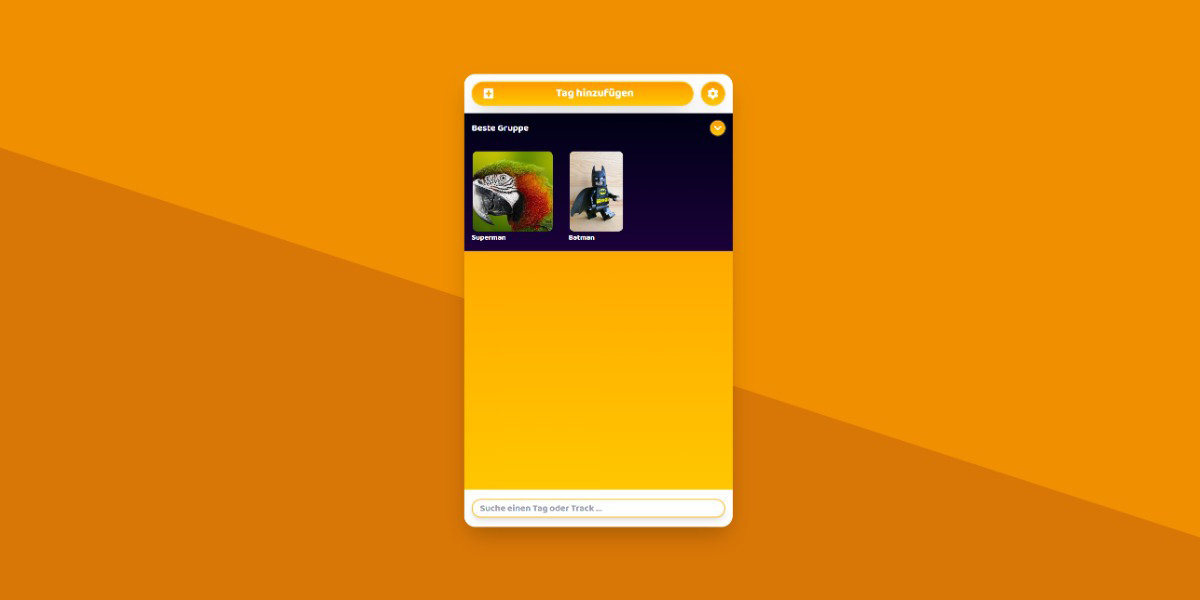
\includegraphics[width=\textwidth]{HomescreenDesktop.jpeg}
    \caption{Desktopansicht}
    \label{fig1}
\end{figure}
Da unsere Anwendung für die mobile Ansicht optimiert wurde, wurde in der Desktop Ansicht die Anwendung als kleineres Fenster im Handy Format angezeigt.
Dieses streckte sich auf höher aufgelösten Bilschirmen zu sehr in die Höhe in Relation zur Breite.
Das wurde angepasst, dass die Relation Breite zu Höhe besser passt.
Auch wurde ein schönerer Hintergrund hinter der eigentlichen Anwendung gesetzt, die auch farblich zur Farbpalette passt.
\\~\\
\paragraph*{Frontend auf Github.io Pages} $~$ \\
\label{FrontendAufGithubIOPages}
Das Frontend ist vom Raspberry Pi zu Github.io Pages umgezogen.
Somit kann der Endnutzer auch ohne Kenntnis der IP-Adresse des Raspberrys auf die Benutzeroberfläche zugreifen
und muss keine weiteren Änderungen an der Netzwerkkonfiguration vornehmen, um von außerhalb des Heimnetzwerkes auf seine \textit{Leek Box} zugreifen zu können.
Die statischen Dateien von GitHub.io werden auf dem Endgerät geladen, sodass die Benutzeroberfläche angezeigt wird.
In dieser kann der Nutzer die von \textit{Ngrok} bereitgestellte Adresse seiner Leek-Box eingeben, woraufhin sich das Endgerät über einen verschlüsselten Tunnel mit dem Backend der Leek-Box verbindet.
Anfäglich wurde diese Adresse jedoch nicht validiert, sodass die Eingabe einer fehlerhaften Adresse, in einem Fehler 404 resultierte.
Bei einem Neustart des Raspberrys auch die ngrok-Instanz eine neue Adresse erhält, die anschließend manuell im \textit{Spotify Developer Dashboard} eingetragen werden muss.
Folglich musste der Nutzer nach jedem Neustart den Browsercache des Endgerätes löschen, um die Adresse der \enquote{neuen} Leek-Box eingeben zu können.
\\~\\

\wrapfiguresafe{r}{0mm}{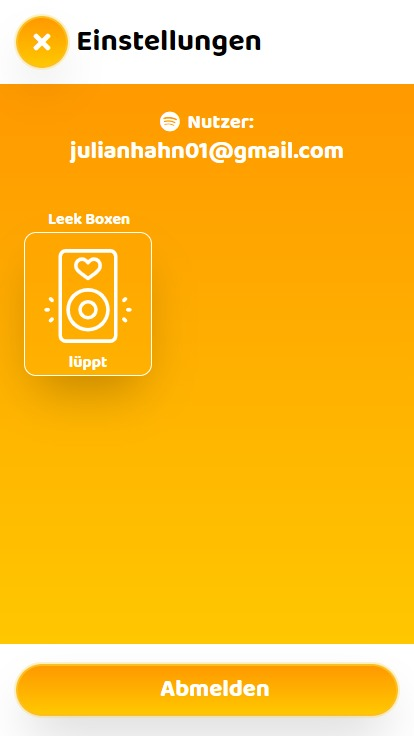
\includegraphics[width=0.45\textwidth]{Settings.jpeg}}{Einstellungen}
\paragraph*{Einrichten einer Leek-Box} $~$ \\
Die Einrichtung einer Leek-Box wurde in diesem Milestone beispielhaft durchgeführt und in einem Setup-Guide dokumentiert. Hierfür wurde auf einem neu aufgesetzten Raspberry Pi Docker installiert
und das auf \textit{DockerHub} verfügbare Backend-Image geladen. Zusätzlich wurde ein \textit{Container} für den angeschlossenen USB-NFC-Reader aus der gleichen Quelle bezogen und gestartet. Dabei
generiert der NFC-Reader eine ID, die im Backend registriert wird. Nach dem Start des Backend-Containers, gibt dieser auf der Konsole eine neue Adresse aus, die von \textit{Ngrok}(vgl. \ref{FrontendAufGithubIOPages})
bereitgestellt wird. Daraufhin kann sich der Benutzer über \url{project-leek.github.io} durch die Eingabe dieser Adresse mit der neuen \textit{Leek-Box} verbinden. Da in der App zu diesem Zeitpunkt noch kein
Lautsprecher hinterlegt wurde, wird der Benutzer automatisch in die Einstellungen umgeleitet. Hier wird die neu angelegte \textit{Leek-Box} zusammen mit der ID angezeigt und bietet dem Nutzer die Möglichkeit den Namen
der Box festzulegen sowie einen vorhandenen Lautsprecher auszuwählen. Der zusätzliche Schritt der Auswahl einer Box wird benötigt, da die Lösung so konzipiert ist, dass ein Nutzer potentiell merhere \textit{Leek-Boxen}
besitzen und die Verwaltung dennoch über ein zentrales Backend erfolgen kann. Somit entfällt die Einrichtung des Backends auf den einzelnen \textit{Leek-Boxen} und muss lediglich einmalig durchgeführt werden.

\paragraph*{Bericht} $~$ \\
Anfänglich wurden die Kapitel und Abschnitte zur Optimierung der Berichtsstruktur überarbeitet.
Die daraus resultierenden Änderungen wurden in Tickets überführt, die sich die einzelnen Teammitglieder zuweisen konnten.
Dies hatte den Vorteil dass, wie schon bei der Softwareentwicklung eine kontinuierliche Übersicht über den Fortschritt der Berichtsarbeit herrschte.
Dadurch, dass das Team sehr viel Freude und Spaß am Entwickeln für das Projekt gefunden hatte, begann die dokumentarische Arbeit schleppend.
Dies hatte zur Folge, dass zum Ende des Sprints nur etwas mehr als die Hälfte des Berichts abgeschlossen war. Somit konnte dem Prüfenden nicht die erste Version des Berichtes vorgelegt werden und das Team bekam somit verspätet erstes Feedback.

\paragraph*{Retrospektive} $~$ \\
Dass der Bericht mit \textit{LaTeX} geschrieben wurde hatte den Vorteil, dass Git sinnvoll genutzt werden konnte und die Änderungen der jeweiligen Mitglieder schnell ersichtlich waren.
So konnte auch weiterhin der Workflow mit \textit{Pull Requests} und zwei \textit{Code Reviews} genutzt werden.

\subsection{Meilenstein 7}
Der finale Meilenstein wurde vom 15.02.2021 bis zum 05.03.2021 angesetzt.

\paragraph*{Letzte Bugfixes} $~$ \\
Neben kleineren Bugfixes, wurde der Fehler behoben, der im letzten Review eine erfolgreiche Präsentation des initialen Verbindens mit der Box verhindert hatte.
Dieser bestand darin, dass der Container des NFC-Readers versuchte, seine \textit{Id} in diesem zu setzen, bevor er eine Verbindung zu dem Backend aufgebaut hatte.
Dies konnte gelöst werden, indem ein \textit{Event-Listener}, der die \texit{Id} in der Datenbank des Backend setzt, auf das \textit{connect}-Event registriert wurde.
Ein weiteren Fehler trat auf, wenn keine Verbindung zur bereits gespeicherten Adresse der \textit{Leek-Box} möglich ist.
Dies trat zum Beispiel auf, wenn die \textit{Leek-Box} nach einem Neustarte eine neue \textit{Ngrok}-Adresse erhielt und resultierte in der Anzeige einer weißen Seite, ohne jegliche Fehlermeldung.
Zur Behebung dieses Problems wurde eine Offline-Seite konzipiert, die Informationen über den Fehler bereitstellt und die Eingabe einer neuen Adresse ermöglicht.


\wrapfiguresafe{r}{0mm}{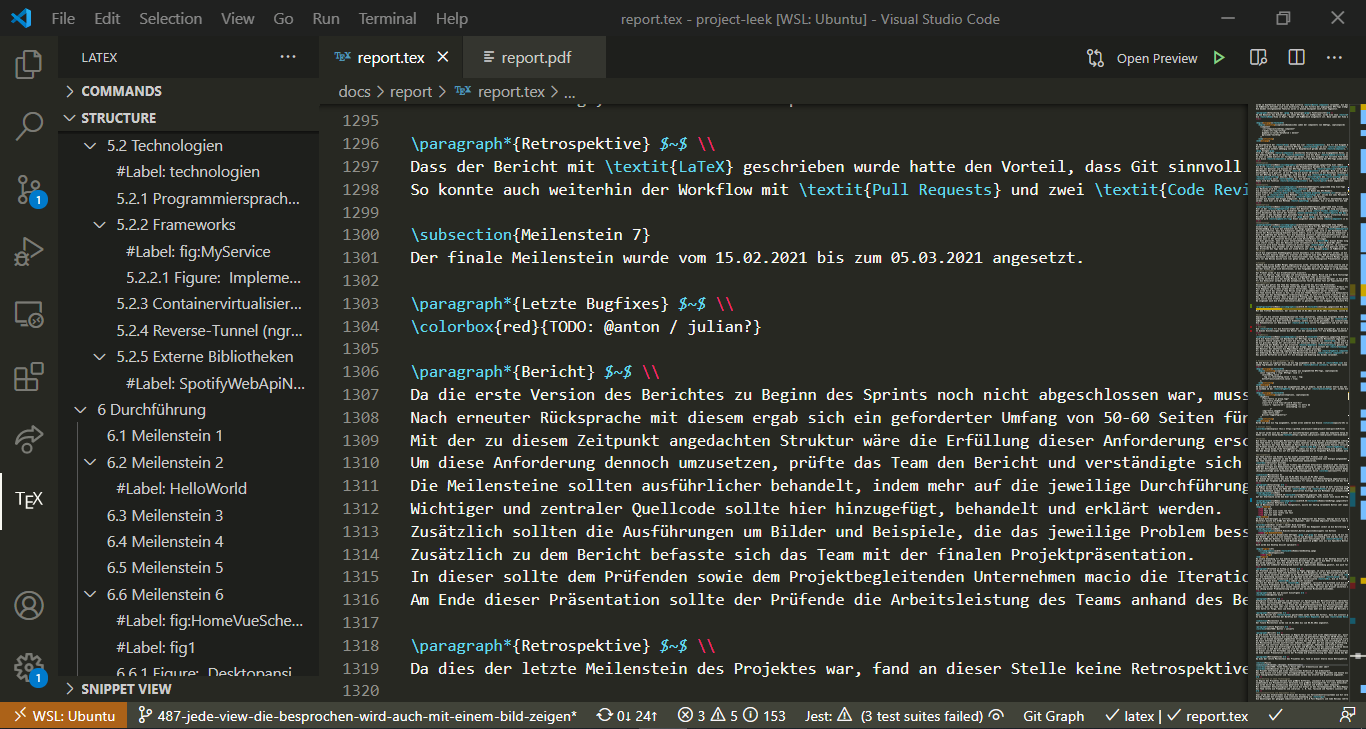
\includegraphics[width=0.65\textwidth]{Latex.png}}{Bericht während der Erstellung}
\paragraph*{Bericht} $~$ \\
Da die erste Version des Berichtes zu Beginn des Sprints noch nicht abgeschlossen war, musste das Team dies zeitig erledigen, um noch erste Anmerkungen vom Prüfenden erhalten und anschließend korrigieren zu können
Nach erneuter Rücksprache mit diesem ergab sich ein geforderter Umfang von 50-60 Seiten für den Bericht (exklusive Anhang).
Mit der zu diesem Zeitpunkt angedachten Struktur wäre die Erfüllung dieser Anforderung erschwert worden.
Um diese Anforderung dennoch umzusetzen, prüfte das Team den Bericht und verständigte sich auf  folgende Änderungen:\\
Die Meilensteine sollten ausführlicher behandelt, indem mehr auf die jeweilige Durchführung und Herangehensweisen eingegangen werden sollte;
Wichtiger und zentraler Quellcode sollte hier hinzugefügt, behandelt und erklärt werden.
Zusätzlich sollten die Ausführungen um Bilder und Beispiele, die das jeweilige Problem besser veranschaulichen ergänzt werden.
Zusätzlich zu dem Bericht befasste sich das Team mit der finalen Projektpräsentation.
In dieser sollte dem Prüfenden sowie dem Projektbegleitenden Unternehmen macio die Iterationen des Projektes und das Produkt präsentiert werden.
Am Ende dieser Präsentation sollte der Prüfende die Arbeitsleistung des Teams anhand des Berichts und der Zufriedenheit des Kunden evaluieren können. Außerdem sollte der Kunde das Produkt selbstständig nutzen und weiterentwickeln können.

\paragraph*{Retrospektive} $~$ \\
Da dies der letzte Meilenstein des Projektes war, fand an dieser Stelle keine Retrospektive statt.

\section{Fazit}
\subsection{Ausblick}
Am Ende der Bearbeitungszeit hat das Team ein Produkt geschaffen, welches die vom Kunden gestellten Mindestanforderungen erfüllt.
Darüber hinaus gibt es noch einige weitere Aspekte der Produktvision, die noch umgesetzt werden könnten.
Darunter befanden sich unter anderem eine Preisbeschränkung der \textit{leek-box}-Hardware auf 30€ und die Möglichkeit eigene Lautsprecher zu nutzen.
Auch die Benutzeroberfläche für die NFC-Tag-Konfiguration könnte noch weiter optimiert werden.
Aber vor allem sollten andere Musikstreaming-Services neben Spotify eingebunden werden,
welche dann in gleicher Weise zur Anmeldung und zum Hinzufügen und Abspielen von Musik genutzt werden.
Nutzer könnten auch ihre Konten bei diesen Services verknüpfen und so NFC-Tags plattformübergreifend gemeinsam verwalten.
Allerdings waren diese Vorstellungen von Anfang an optional, sie bildeten aber die allgemeine Produktvision und legten die Grundlage für mögliche Weiterentwicklung.
Das Team hofft, dass Teile der Open-Source-Community genug Interesse an diesem Projekt haben werden, um daran weiter zu entwickeln.
Vielleicht haben diese auch weitere Ideen für die Zukunft der \textit{leek-box}.
Des weiteren besteht auch die Hoffnung, dass macio einiges von der Organisation dieses Projekts gelernt hat und auch fortlaufend weiter daraus lernen wird.
So könnten dort in Zukunft auch weitere Projekte als Open-Source aufgestellt werden.
Auch hofft das Team, dass auch in den nächsten Jahren des \glqq Projekt Informatik \grqq{} mehr Open-Source Projektvorschläge gestellt werden.
Dies würde Studierende damit konfrontieren Software zu erstellen, die nicht zwingend abgeschlossen wird.
Sie würden auch lernen, Code für unbekannte Kollaborierende zu schreiben.
Vor allem würde es aber zeigen, wie viel Spaß lebendige und langlebig angelegte Projekte machen können.

\subsection{Projektreflexion}
Das Projekt Informatik gab einen realistischen Einblick in die Arbeitswelt.
Das Team musste sich klassischen Alltagsproblemen stellen, Lösungswege finden und konnte wichtige Erkenntnisse für die Zukunft daraus ziehen.
Auch Coding-Entwurfsmuster und -Konventionen wurden neu erlernt und praktisch angewandt.
$~$ \\
%Einarbeitung in neue Technologien
Zu Beginn des Projektes bestand eine größere Differenz, inwieweit die einzelnen Teammitglieder mit den jeweiligen Technologien vertraut waren.
Insbesondere die Projektstruktur bereitete eine größere Einstiegshürde für viele Entwickler.
Sie wurde durch das automatische generieren von Dateien und Ordnern immer komplexer.
Mit zunehmender Entwicklungszeit und durch die Arbeit an den Teilkomponenten des Mono-Repositorys gewannen die Entwickler jedoch schnell mehr Überblick über die Struktur.
Das Team lernte wie Frameworks und Libraries  z. B. Vue, Tailwind und Feathers sinnvoll und hilfreich eingesetzt werden können.
$~$ \\
%Versionskontrolle und Deployment Cycle
Zwar wurde den Studierenden im Studium der Vorteil von Versionskontrollsystemen wie Git vermittelt, doch fand sich selten ein praktisches Anwendungszenario, dass Git über die Hauptfunktion der Versionierung hinaus sinnvoll genutzt hat.
Dieses Projekt bot erstmals eine sinnvolle Anwendung von \textit{git}.
Die Umsetzungen der gängigen Industriestandarts we z.B Pull-Requests und Code Reviews lehrte uns die Vorteile von Git in einer komplexen Umgebung.
Diese Methoden führten zu folgenden maßgebliche Verbesserungen:
Mit zwei erfordelichen Code Reviews pro Pull Request, konnten Fehler im Code häufiger entdeckt werden und so eine höhere Codequalität erreicht.
Als positiver Nebeneffekt konnten die Reviewer außerdem während des Prozesses neue Funktionen und Codemuster erlernen, zu denen sie bei Bedarf (per Kommentar) Fragen stellen konnten.
Die Gewöhnung an diesen Deployment Cycle brauchte eine gewisse Zeit, fand aber von Sprint zu Sprint immer mehr Wertschätzung im Team.
$~$ \\
%Automatisierte Tests und Deployment
Jeder Pull Request durchlief mehrere automatisierte Tests - sogenannte \textit{Actions} - die den geänderten Code auf Korrektheit in Syntax und simplen Semantischen fragen getestet haben.
Inhaltliche Funktionen der Applikation wurden durch die Tests nicht abgedeckt.
Diese prüften den Quellcode anhand fest eingestellter Testparameter.
Durch diese Tests wurde dem Team viel manuelle Arbeit abgenommen und die Fehlerquelle Mensch minimiert.
Änderungen im Master werden automatisch verarbeitet. Die neue Version des Codes wird auf Github.io veröffentlicht und geänderte Latex Dateien als PDF im eigenen Branch erstellt.
Für Pull Requests wurde ebenfalls eine Vorschau erstellt und auf einer separaten Webseite veröffentlicht.
Dank dieser Automatisierungen konnte sich das Team mehr auf das Weiterentwickeln des Projektes konzentrieren.

%Regelmäßige Standups und Retrospektiven
Durch die regelmäßigen Standups entstand ein Ort für den Austausch von Problemen und Informationen über Fortschritt und neue Funktionen.
So wurde verhindert, dass Probleme untergingen, neues Wissen wurde schneller verbreitet und die gesamte Teamproduktivität verbessert.
Das bei den Retrospektiven entstandene Feedback erwies sich als sehr wichtig für das Teamklima.
Auch die hierbei angesprochenen Probleme und Verbesserungsvorschläge wurden vom Team als sehr wertvoll für die nächsten Sprints erkannt und entsprechend adaptiert.

%Kommunikation und Eigeninitiative
Anfänglich hat sich das Team zu sehr auf die Standups, als alleiniges Kommunikationsmittel verlassen, wodurch die Absprache zwischen den Teammitgliedern nur selten statt gefunden hat.
Der Umfang erster Tickets war deutlich zu groß.
Die Komplexität eines Tickets hat Teammitglieder davon abgehalten sich mit der Thematik zu beschäftigen.
Da konkrete Fragen bei einem gänzlich neuen Thema schwierig zu formulieren sind, wurde oft komplett auf Hilfe verzichtet und das Ticket zur Seite gelegt.
Lösungsansätze wurden gemeinsam in den Retrospektiven erarbeitet.
Weiterhin konnte offen über Probleme gesprochen werden, indem teaminterne Evaluationen stattgefunden haben.

%Planung, Zielsetzung und Einschätzung
Größere Probleme hatte das Team mit dem Zeitmanagement der einzelnen Ticket.
Während eines Milestones wurden manchmal nicht alle geplanten Tickets fertiggestellt, oder es wurde nachträglich zu viel in den Sprint neu Aufgenommen.
Beides resultierte in Überstunden und zu wenig Zeit fürs Testen am Ende eines Meilensteins.
Aus diesen Erfahrungen, hat das Team gelernt wie wichtig es ist die Planung des Meilensteins und dessen Tickets besonders sorgfältig zu gestalten.
So hat das Team sich auch vorgenommen, mindestens zwei Tage vor einem Sprintende alle für den Sprint benötigten Tickets fertiggestellt zu haben.
Dadurch sollte genügend Zeit geschaffen werden, um Tickets auf Korrektheit zu testen und konfliktfrei in den Master Branch mergen zu können.
Auch wenn die Lösung dieses Problem hätte effizienter behandelt werden können, war diese Methode angesichts der knappen Projektlaufzeit die effektivste.


\end{onehalfspace}

\newpage
\section{Anhang}
\label{pdf:macioprojektskizze}
\label{FigmaDesigns}
\label{FlowCharts}
\label{anhang:lucidchart}
\printbibliography
\end{document}
